\documentclass[notes]{beamer}
\usetheme{Madrid}
\usepackage[utf8]{inputenc}
\usepackage{amsmath, amssymb}
\usepackage{graphicx}
\usepackage{subcaption}
\usepackage{tikz}
\usepackage{stmaryrd}
% \setbeameroption{show notes on second screen=right}
\title{A dynamical perspective on QEC}
\subtitle{Using ZX/W rewrites to go beyond depolarizing noise}
\author{Clemens Schumann}
\date{\today}

\begin{document}

\begin{frame}
  \titlepage
\end{frame}

\begin{frame}{Outline}
  \tableofcontents
\end{frame}

\section{Motivation}
\begin{frame}
  \centering
  \Huge \insertsection
\end{frame}
\begin{frame}{Motivation}
    \begin{itemize}
        \item QEC codes described in the stabilizer formalism not directly implementable, either due to the \textbf{weight} of operators or 
        the required \textbf{connectivity} on qubits
        \item Real-world implementations require intermediary steps in the measurement of stabilizers\\\hspace{0.5cm} $\Rightarrow$ \textbf{Syndrome extraction}
        
    \end{itemize}
\end{frame}
\begin{frame}{Motivation}
    \begin{itemize}
        \item Modeling Errorchannels, detectors, corrections in a diagramatic representation can expose symmetries as patterns
        for simplification routines\\
        \hspace{1em} $\Rightarrow$ We could feed our problems into a compiler
        \item In many ways, both hardware tailoring and QEC itself are just compilation problems
        
    \end{itemize}
\end{frame}

\section{ZX and rewrites}
\begin{frame}
  \centering
  \Huge \insertsection
\end{frame}

\begin{frame}{ZX}
    ZX is a monoidal category whose objects are spiders and whose morphisms are called "rewrite rules"
    % \begin{itemize}
    %     \item ZX is a monoidal category whose objects are spiders and whose morphisms are called "rewrite rules"
    %     % \item Z and X represent a frobenius algebra on the object of quantum maps
    %     % \item algebraic axioms on those result in core rewrite rules
    % \end{itemize}
    \begin{figure}
        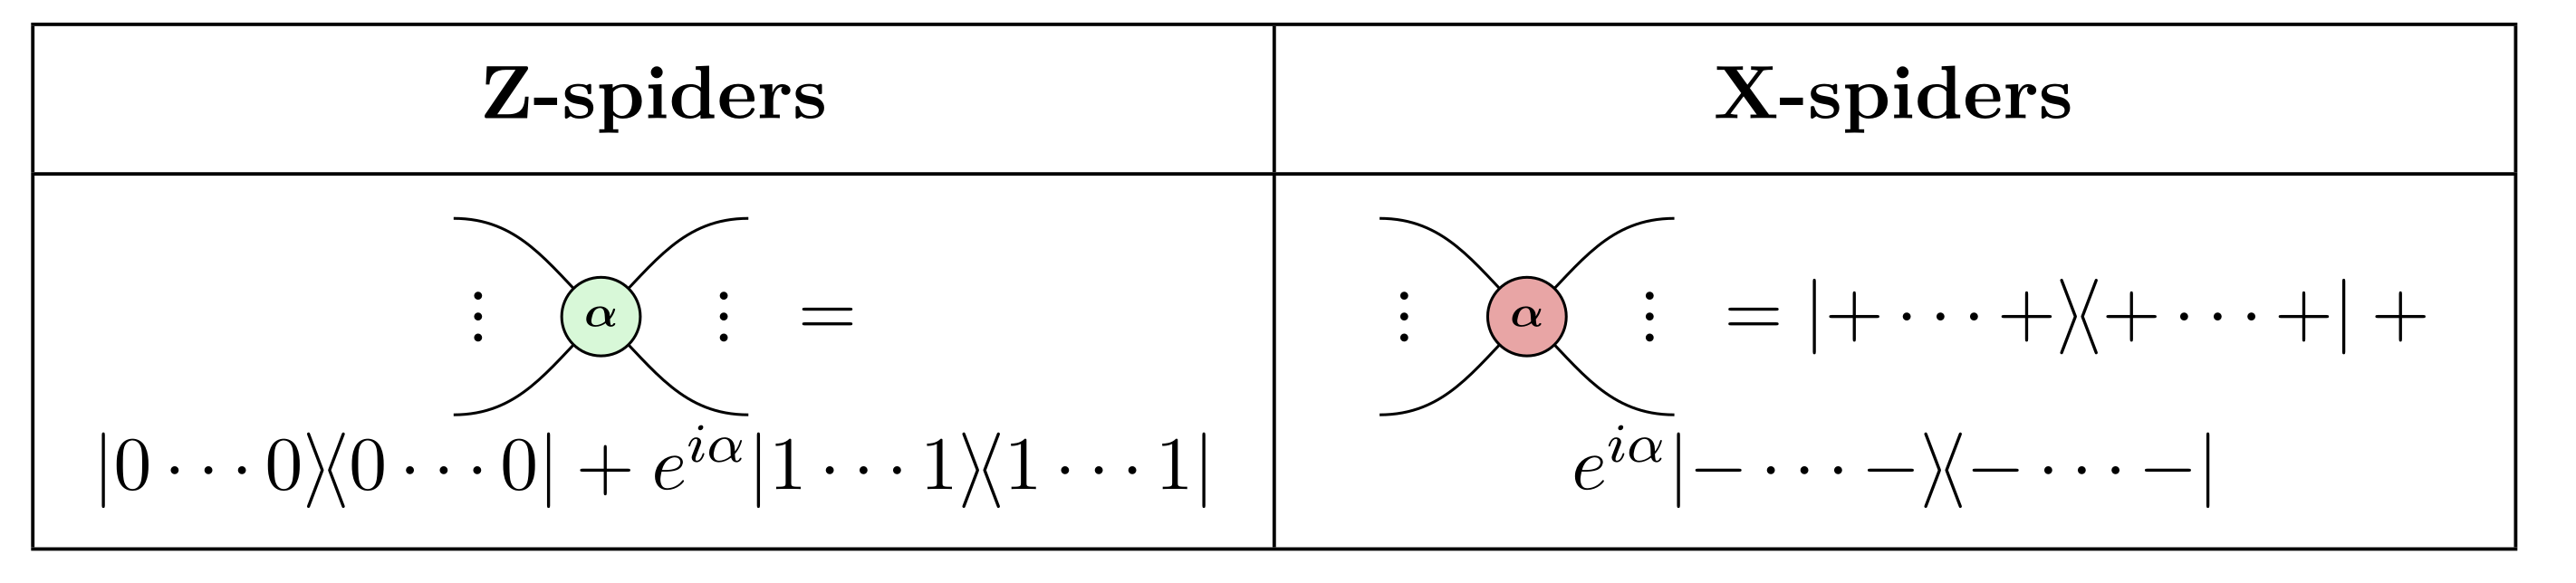
\includegraphics[width=0.9\textwidth]{img/spiders.png}
        \label{spiders}
        \caption{(unnormalized) Z and X spider definitions}
    \end{figure}
\end{frame}

\begin{frame}{Core ZX rules}
    \begin{columns}
        \begin{column}{0.45\textwidth}
            \begin{itemize}
        \item Equality of any two diagrams $D_1$ and $D_2$ can be proven using a generating set 
        of local rewrite identities.
        % \item Generating rewrite rules
        \end{itemize}
        \end{column}
        \begin{column}{0.55\textwidth}
            \begin{figure}
                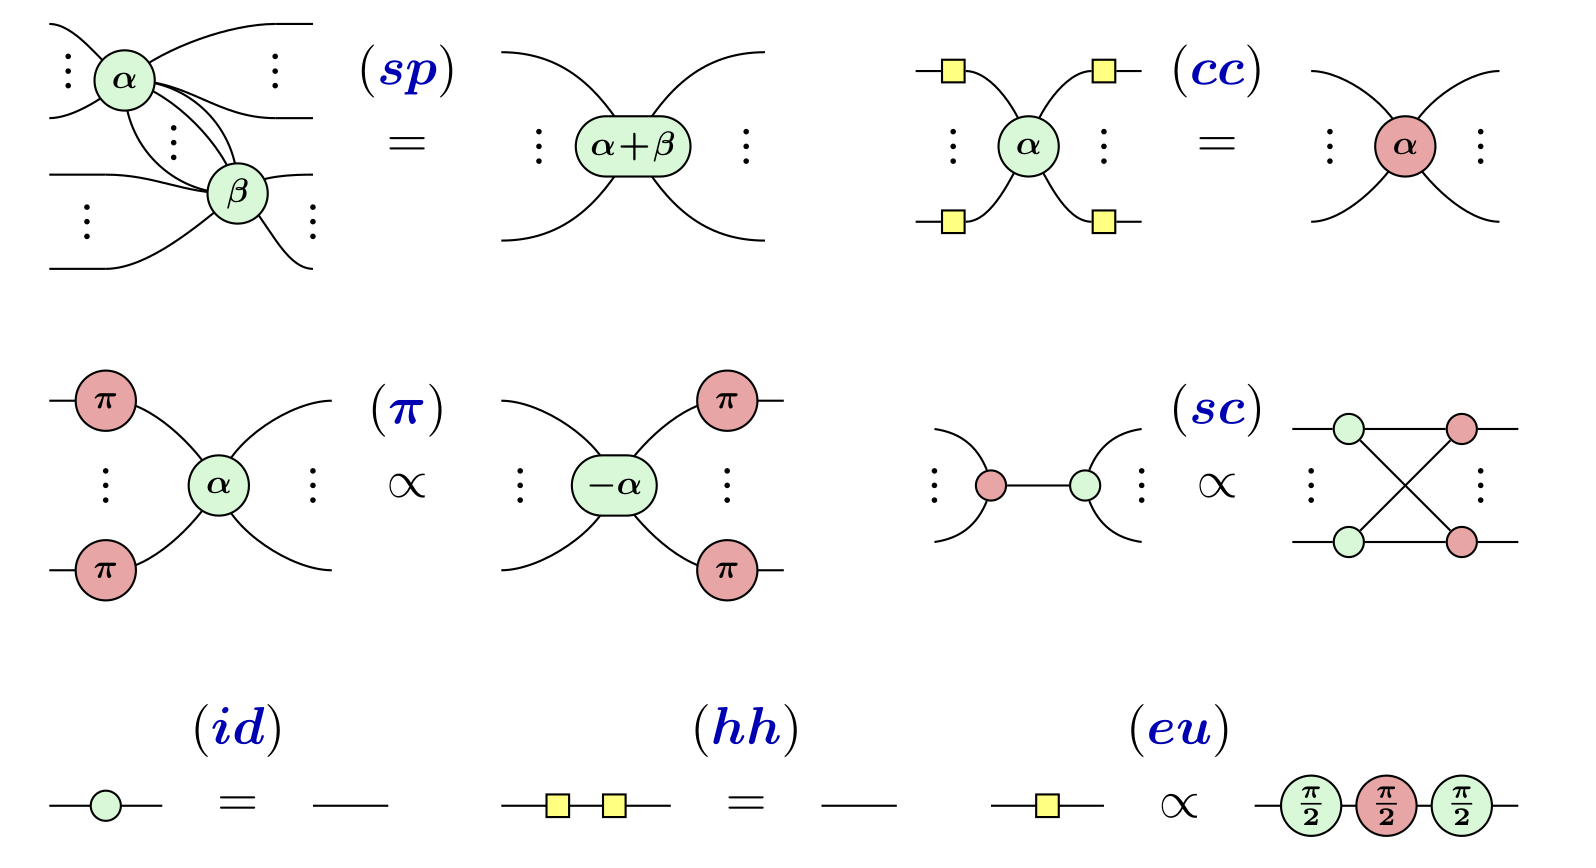
\includegraphics[width=1\textwidth]{img/rewrites.png}
                \caption{Generating set of 7 local rewrite identities}
            \end{figure}
        \end{column}
    \end{columns}
\end{frame}

\section{Teleportation}
\begin{frame}
  \centering
  \Huge \insertsection
\end{frame}
\begin{frame}{Teleportation protocol}
    \begin{figure}
        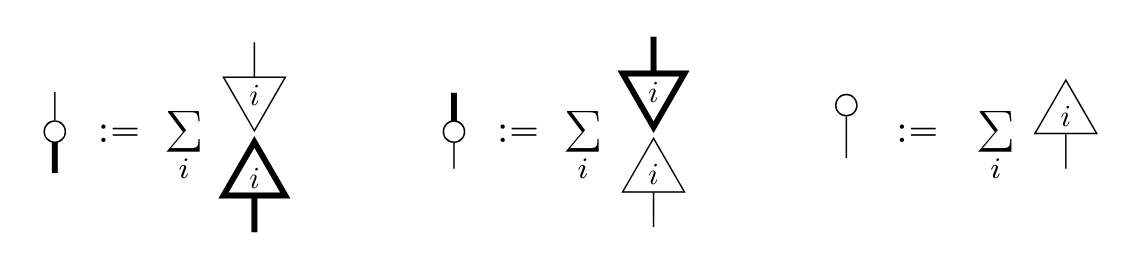
\includegraphics[height=0.2\textheight]{img/stringMeas.png} 
    \end{figure}
    \begin{figure}
        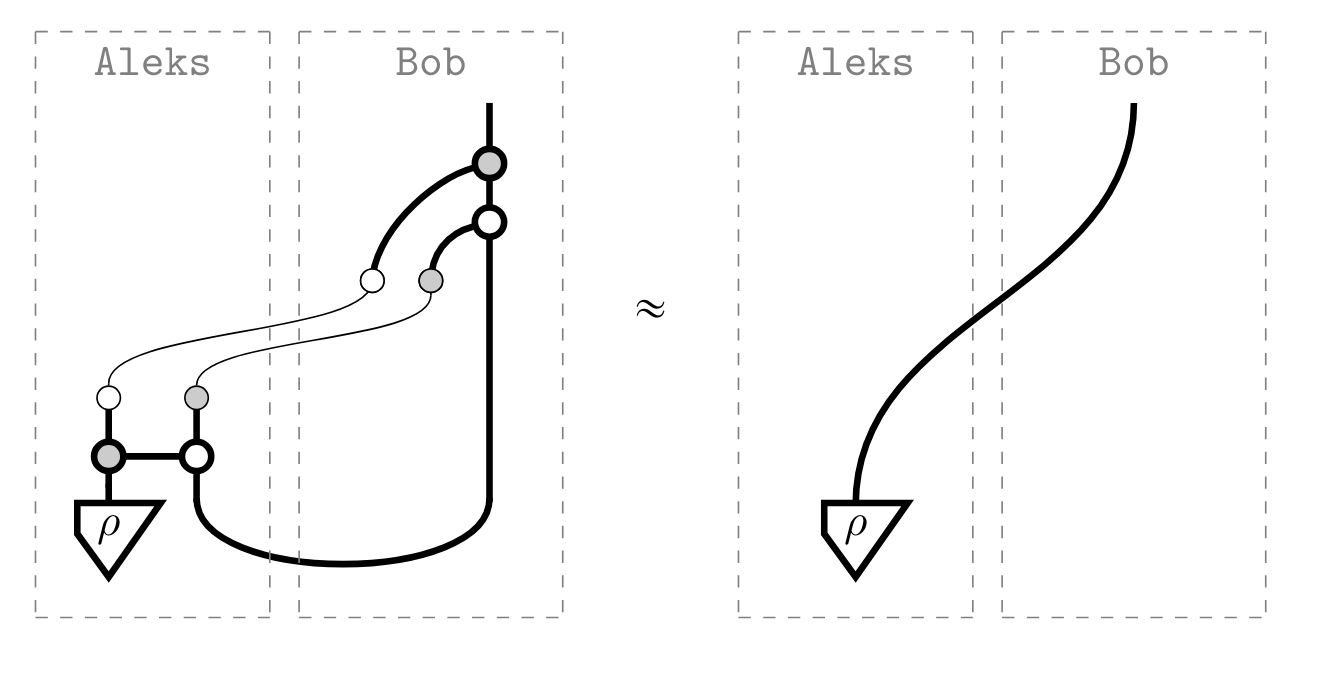
\includegraphics[height=0.45\textheight]{img/stringTele.png} 
        \caption{In the teleportation protocol, the classical in/outputs are $\delta$-functions, 
        which is why sometimes they are just denoted with a and b labels}
    \end{figure}
\end{frame}


\begin{frame}{Pauliwebs}
    \begin{itemize}
        \item Pauliwebs are syntactic sugar to ZX diagrams, used to track local gauge symmetries on a diagram
        \item For the Clifford fragment of ZX, i.e. diagrams whose spiders only have phases in integer multiples of $\frac{\pi}{2}$, 
        two conditions must hold locally for every spider:
        \begin{itemize}
            \item[$-$] a spider with $k\pi$ phase can have
            \begin{enumerate}
                
                \item An even number of legs marked in its own color and/or
                \item All or none of its legs marked in opposite color 
            \end{enumerate}
            \item[$-$] a spider with $\pm\frac{\pi}{2}$ phase can have
            \begin{enumerate}
                \item An even number of legs marked in its own color and none in the opposite color
                \item An odd number in its own color and all legs in the opposite color
            \end{enumerate}
        \end{itemize}  
    \end{itemize}
\end{frame}

\begin{frame}{Pauliwebs: Examples}
    \begin{figure}
        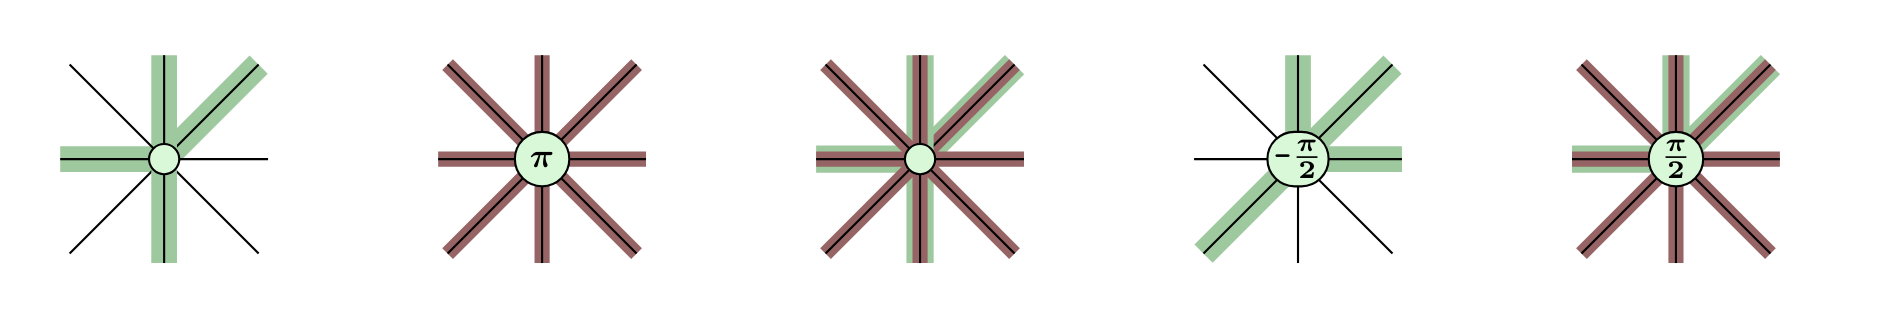
\includegraphics[width=\textwidth]{img/pauliwebs.png}
        \caption{Examples of valid Pauliwebs. Each of these is semantically 
        equivalent to the underlying spider without any webs}
    \end{figure}
\end{frame}

\begin{frame}{Pauliwebs: Examples}
    \begin{figure}
        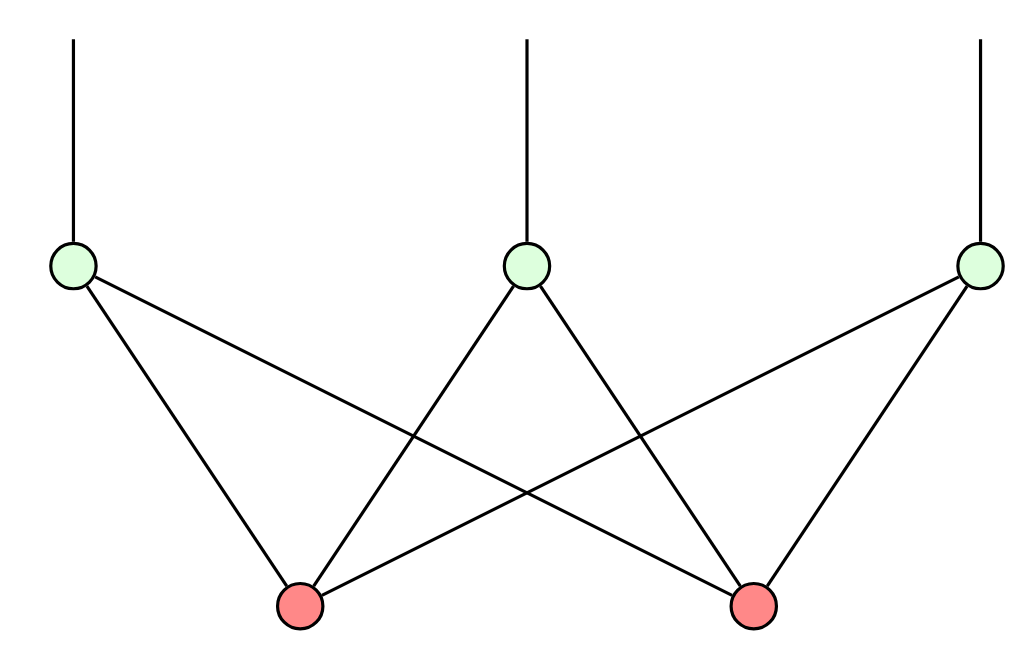
\includegraphics[height=0.7\textheight]{img/paulistate.png}
        \caption{Using pauliweb firings, we can read off the stabilizers of this stabilizer state.}
    \end{figure}
\end{frame} 

\section{The QEC perspective}
\begin{frame}
  \centering
  \Huge \insertsection
\end{frame}
\begin{frame}{Detectors}
    \begin{itemize}
        % \item Problem with this might be high incidence on tanner graph;
        % \item in the full picture there is significant overlap btw detectors, they are heavily connected
        % \item maybe this is just a feature of color codes though?
        \item A detector is a set of measurements outcomes whose joint parity is promised to be even in the absence of a detection event.
        \item Simplest case: Measuring a stabilizer element twice
        \begin{itemize}
            \item If $S_i\in S$ then $(M_{S_{i,1}} + M_{S_{i,2}})\text{mod}2=0$ in the absence of the detectable error $E_i$ for that detector  
            \item This follows from $\forall S_i, S_j \in S: [S_i,S_j]=0$ and $\forall E_i \in E_{detectable}: \exists S_i\in S: \{E_i,S_i\}=0$
        \end{itemize}
        \item But: more complex detector configurations involving 3 or more measurements possible
    \end{itemize}
\end{frame}

\begin{frame}
    \begin{figure}
        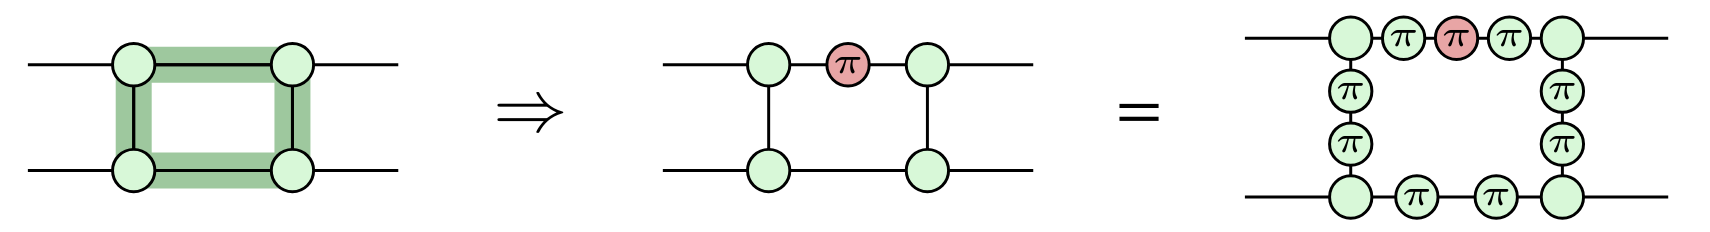
\includegraphics[width=\textwidth]{img/detectorProof1.png}
        \makebox[\textwidth][l]{%
      \hspace{2.5cm} % Adjust this to shift right
      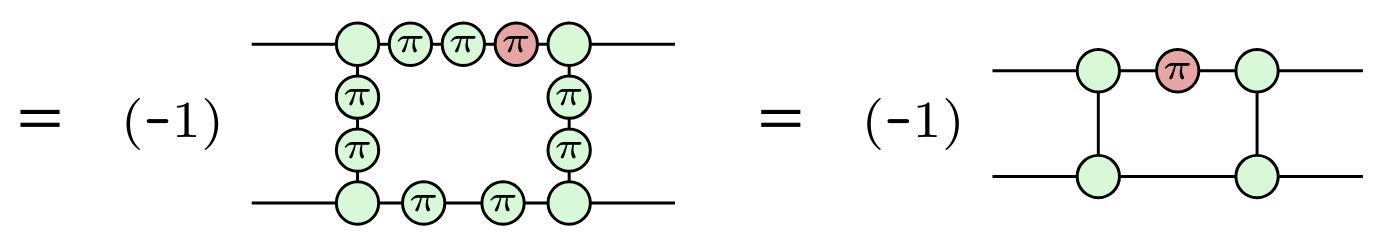
\includegraphics[width=0.8\textwidth]{img/detectorProof2.png}
    }
    \caption{A diagram D that can be rewritten to -D is equal to 0.}
    \end{figure}
    \hspace{5em}$\Rightarrow$ The map described by the diagram cannot occur.
\end{frame}

\begin{frame}
    \begin{figure}
        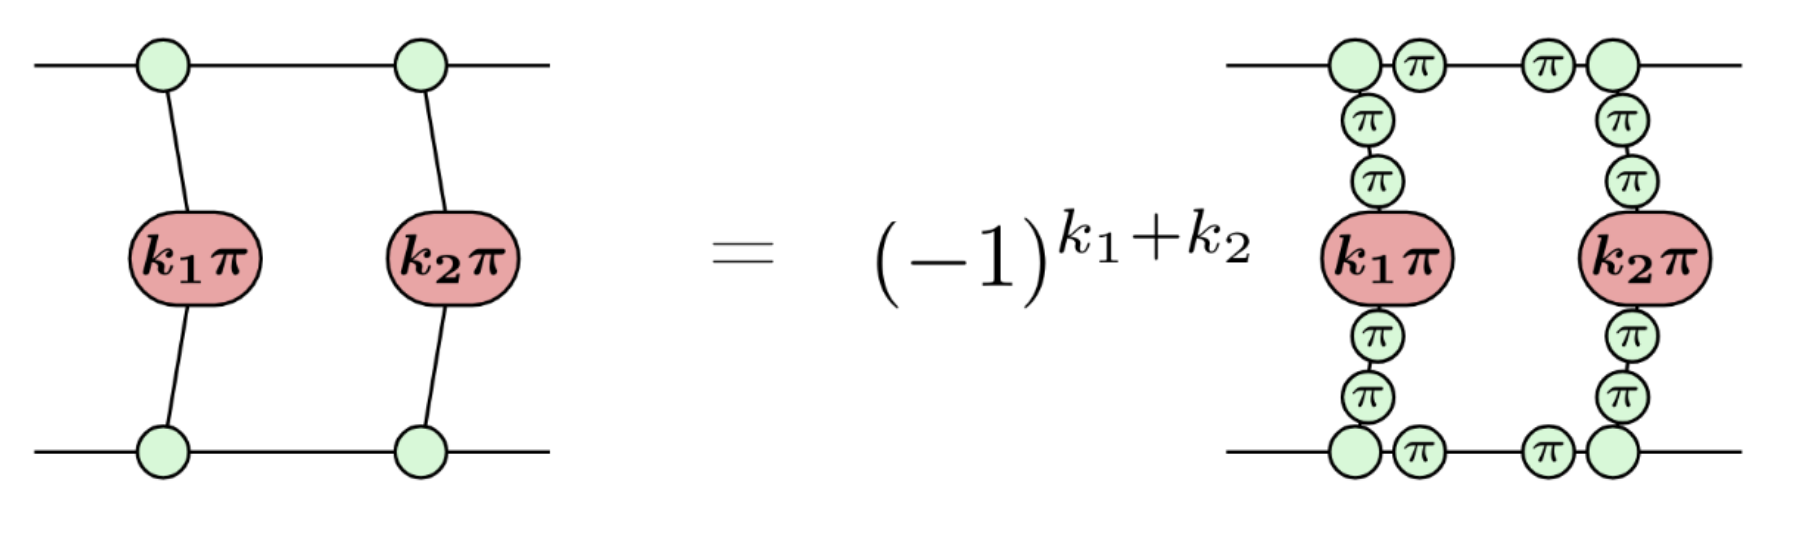
\includegraphics[width=\textwidth]{img/fullDetectorProof1.png}
        \makebox[\textwidth][l]{%
      \hspace{4.48cm} % Adjust this to shift right
      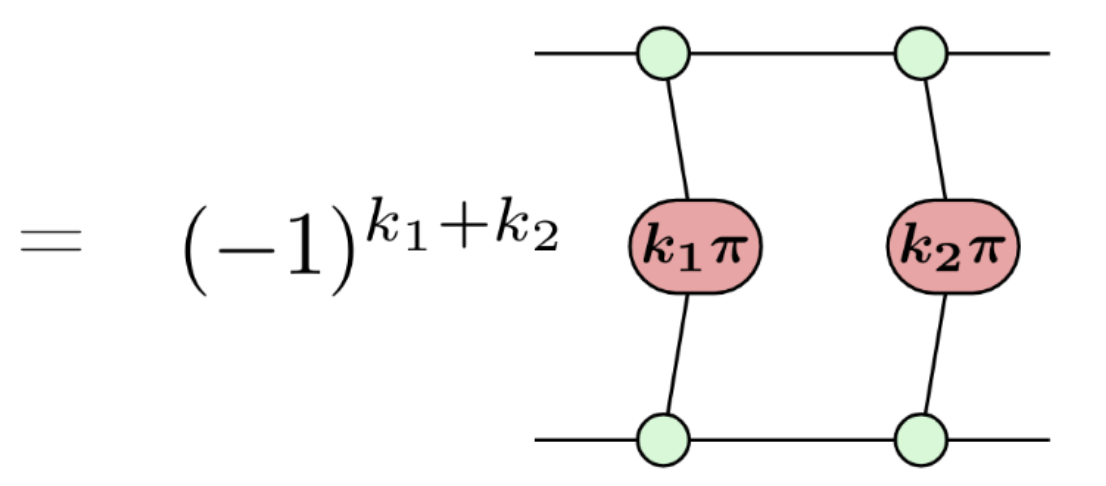
\includegraphics[width=0.6\textwidth]{img/fullDetectorProof2.png}
    }
    \caption{Case with general measurement results $k_1$ and $k_2$.}
    \end{figure}
    \hspace{5em}$\Rightarrow$ The map described by the diagram cannot occur.
\end{frame}

\begin{frame}{Distance preservation}
    \begin{itemize}
        \item ZX distance: smallest nontrivial error $\mathcal{E}$ s.t. $\llbracket D+\mathcal{E} \rrbracket\neq 0$.
        \item A \textbf{distance-preserving} rewrite, is a rewrite that preserves ZX distance.
    \end{itemize}
\end{frame}

\begin{frame}{Distance preservation}
    \begin{figure}
        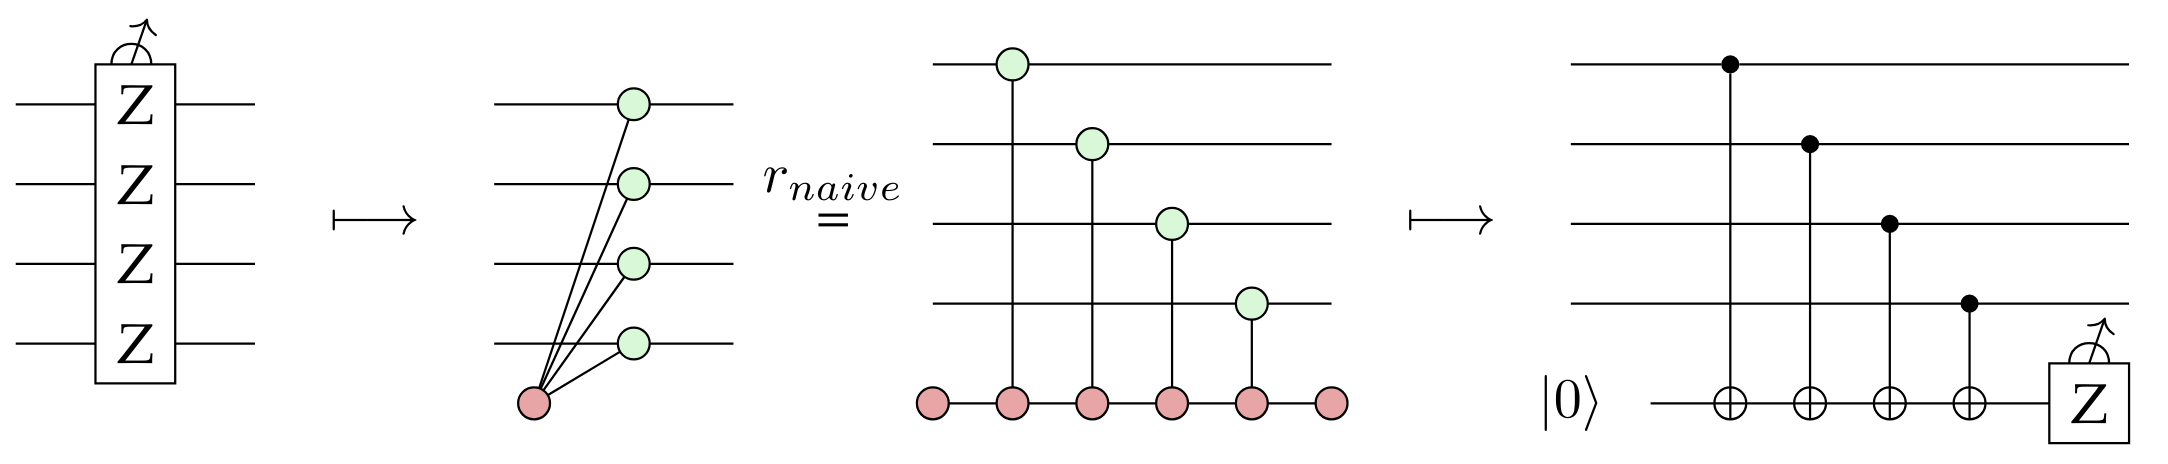
\includegraphics[width=\textwidth]{img/naiveRewrite.png}
        \caption{example of a naive non-distance-preserving rewrite/ circuit extraction}
        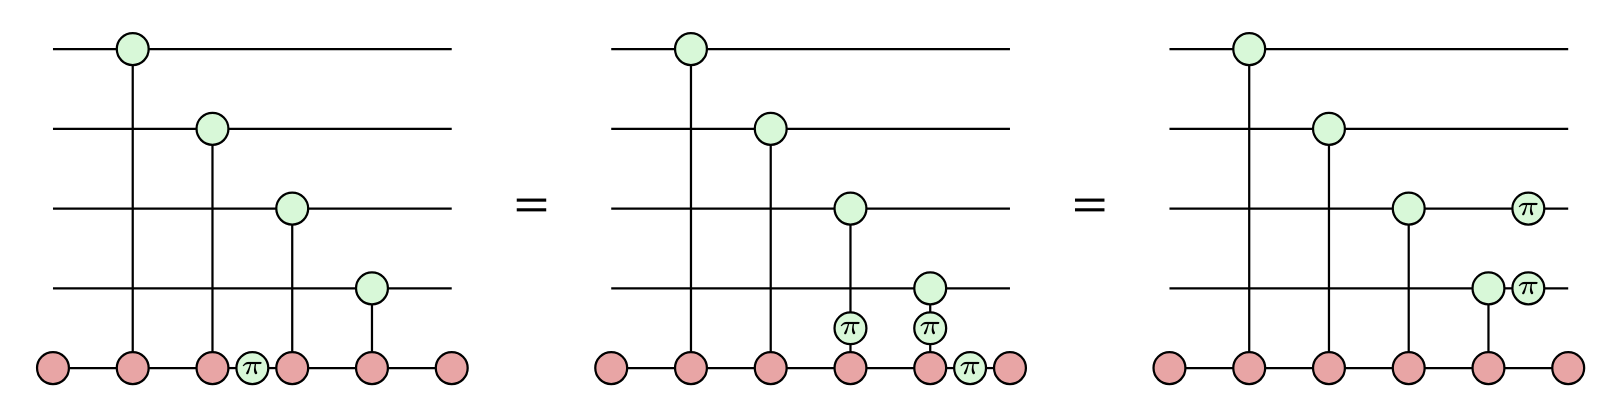
\includegraphics[width=\textwidth]{img/naiveConsequences.png}
        \caption{Errors propagate onto multiple qubits under this naive rewrite}
    \end{figure}
\end{frame}

\begin{frame}{Distance preservation}
    These two rewrites are enough to distance-preservingly rewrite arbitrary-legged spiders:
    \begin{figure}
        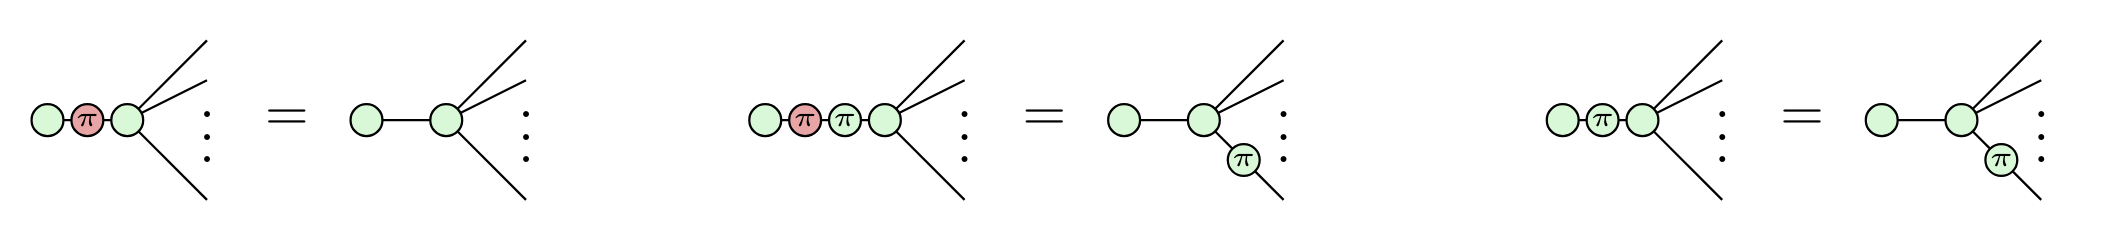
\includegraphics[width=\textwidth]{img/fuse.png}
        \caption{Unfusing a dangling leg is distance-preserving}
        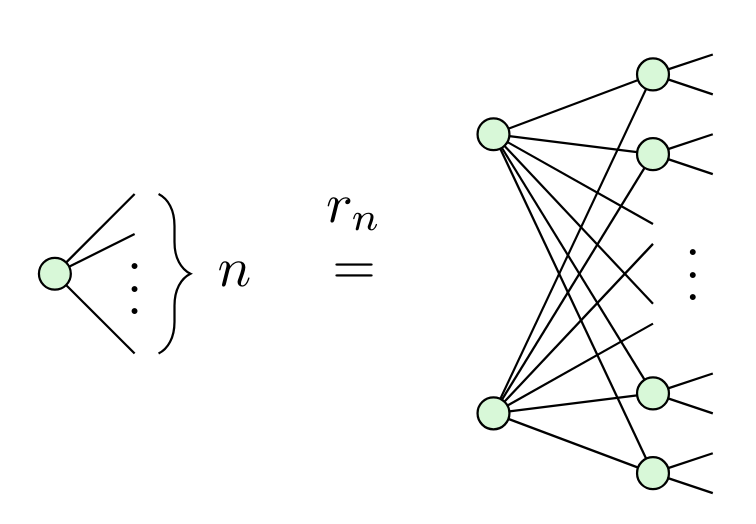
\includegraphics[height=0.35\textheight]{img/distpres.png}
        \caption{Distance-preserving rewrite of a spider with n legs where n mod 2 = 1}
    \end{figure}
    
\end{frame}

\begin{frame}{Detectors: ZX example}
    \begin{figure}
        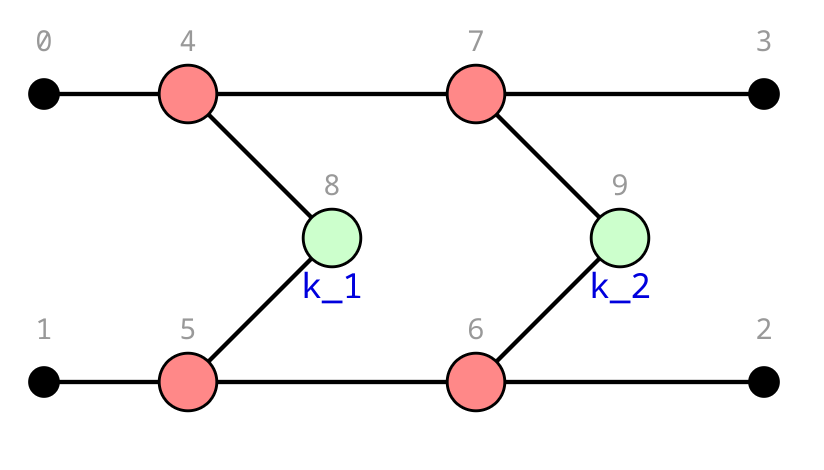
\includegraphics[width=0.6\textwidth]{img/xxStab.png}
        \caption{Two consecutive XX measurements. The parity of $k_1$+$k_2$ will be even in the absence of errors.}
    \end{figure}
\end{frame}
\begin{frame}{Detectors: ZX example}
    \begin{columns}
        \begin{column}{0.4\textwidth}
            \begin{itemize}
                \item A ZX diagram representing the Choi state of two consecutive XX measurements, 
                brought into bipartite form
            \end{itemize}
            
        \end{column}
        \begin{column}{0.6\textwidth}
            \begin{figure}
                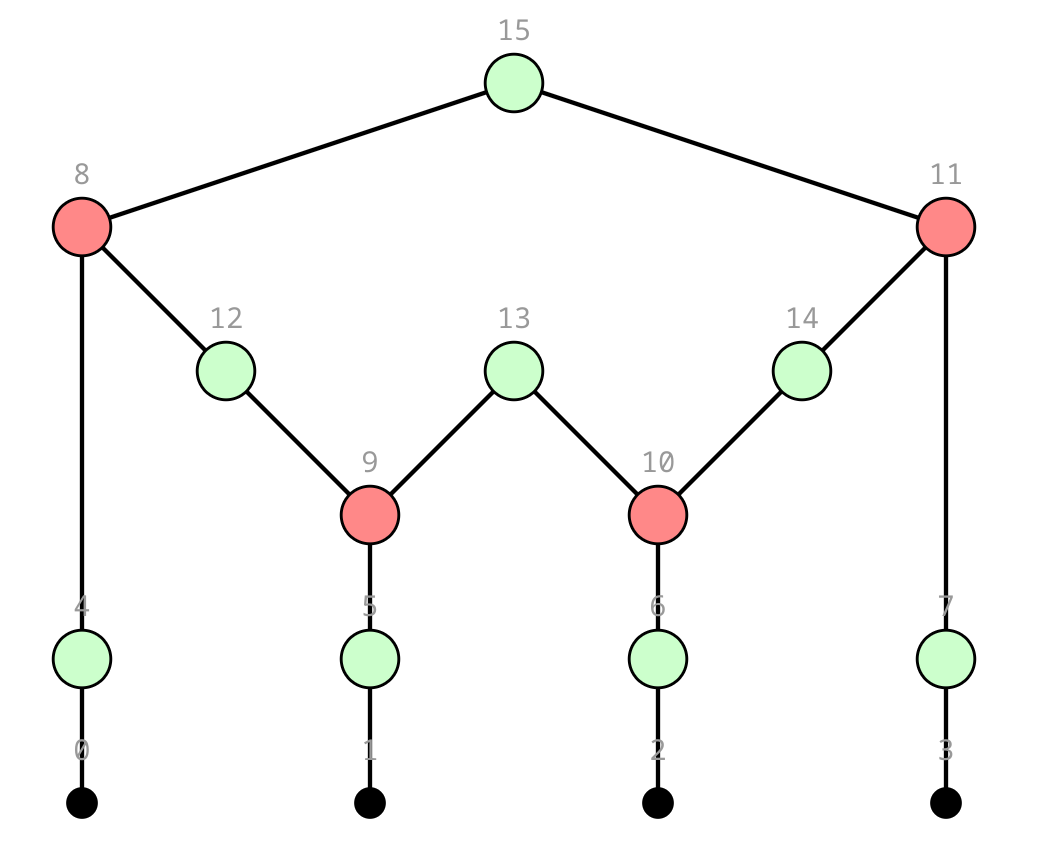
\includegraphics[width=\textwidth]{img/xxStabChoi.png}
                \caption[]{two XX measurements Choi state ($k_1$ and $k_2$ on 12 and 14)}
            \end{figure}
            
            
        \end{column}
    \end{columns}
\end{frame}

\begin{frame}{Firing verification matrix}
    Bringing the graph into bipartite form, the conditions for phaseless 
    diagrams now simplify to:
    \begin{enumerate}
        \item Every internal spider must have an even number of neighboring spiders firing
        \item Output spiders cannot fire
    \end{enumerate}
    % \\
    % \emph{Every spider must have an even number of neighboring spiders firing}
    % \\
    A firing vector is therefore \textbf{valid} if for all internal spiders q it satisfies
    \begin{equation}
        \sum_{x:(q,x)\in E} \textbf{x} = \text{0 mod 2}
    \end{equation}
    We can encode this in a \textbf{Firing verification matrix},
    whereby we want our firing vectors to satisfy $M_D \vec{v}=0$ with: 
    \begin{equation}
        M_D = \left( \begin{array}{c|c}
            I_n & \raisebox{-1.7ex}{N} \\
            \emptyset & 
            \end{array} \right)
    \end{equation}
\end{frame}

\begin{frame}{Firing verification matrix (non-CSS)}
    For more general non-CSS stabilizer codes, $\pm \frac{\pi}{2}$ spiders are needed in their diagrams.\\
    In order to account for $\pm i$ phases accrued by firing, internal spiders h with phase $\pm \frac{\pi}{2}$ must then additionally satisfy:
    \begin{equation}
        \sum_{x:(h,x)\in E} \textbf{x} = \text{h mod 2}
    \end{equation}
    giving us an updated verification matrix
    \begin{equation}
        M_D = \left( \begin{array}{c|c}
            I_n & \raisebox{-1.7ex}{N} \\
            \emptyset & 
            \end{array} \right)
            - \left( 
                \begin{array}{c|c}
                    \emptyset & \emptyset \\
                    \emptyset & I_r
                \end{array}
            \right)
    \end{equation}
    where r is the number of internal $\pm \frac{\pi}{2}$ spiders.
    
\end{frame}

\begin{frame}{Computing Detection Webs on a CSS code}
    \begin{columns}
        \begin{column}{0.4\textwidth}
            \begin{itemize}
                \item Fire spiders in their opposite color according to \textbf{valid firing vector}
                
            \end{itemize}
        \end{column}
        \begin{column}{0.6\textwidth}
            \begin{figure}
                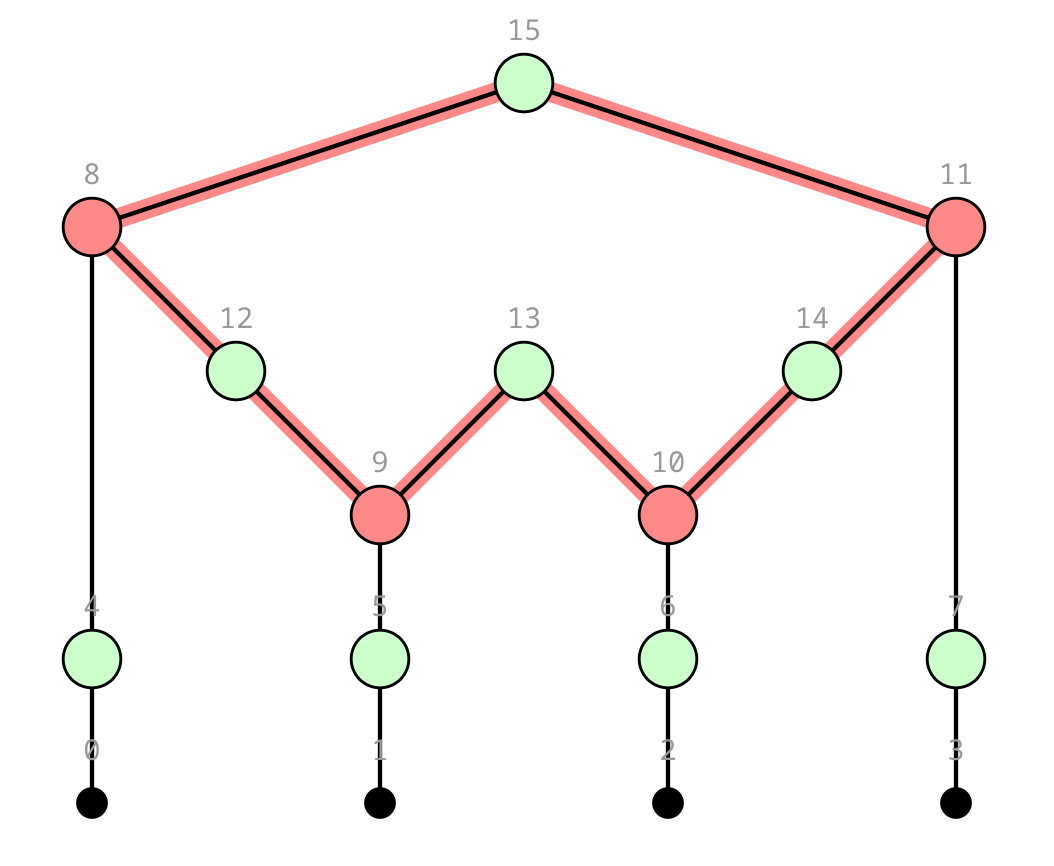
\includegraphics[width=0.8\textwidth]{img/firing.png}
                \caption{Fired spiders 8, 9, 10 and 11}
            \end{figure}
            
        \end{column}
    \end{columns}
    
\end{frame}

\section{Some rewrites and their detection webs}
\begin{frame}
  \centering
  \Huge \insertsection
\end{frame}
\begin{frame}{Example: Dist-pres rewritten XXX measurement}
    \begin{columns}
        \begin{column}{0.4\textwidth}
            \begin{itemize}
                \item Detection webs give a more circuit-level understanding of noise
            \end{itemize}
            
        \end{column}
        \begin{column}{0.55\textwidth}
            \begin{figure}
                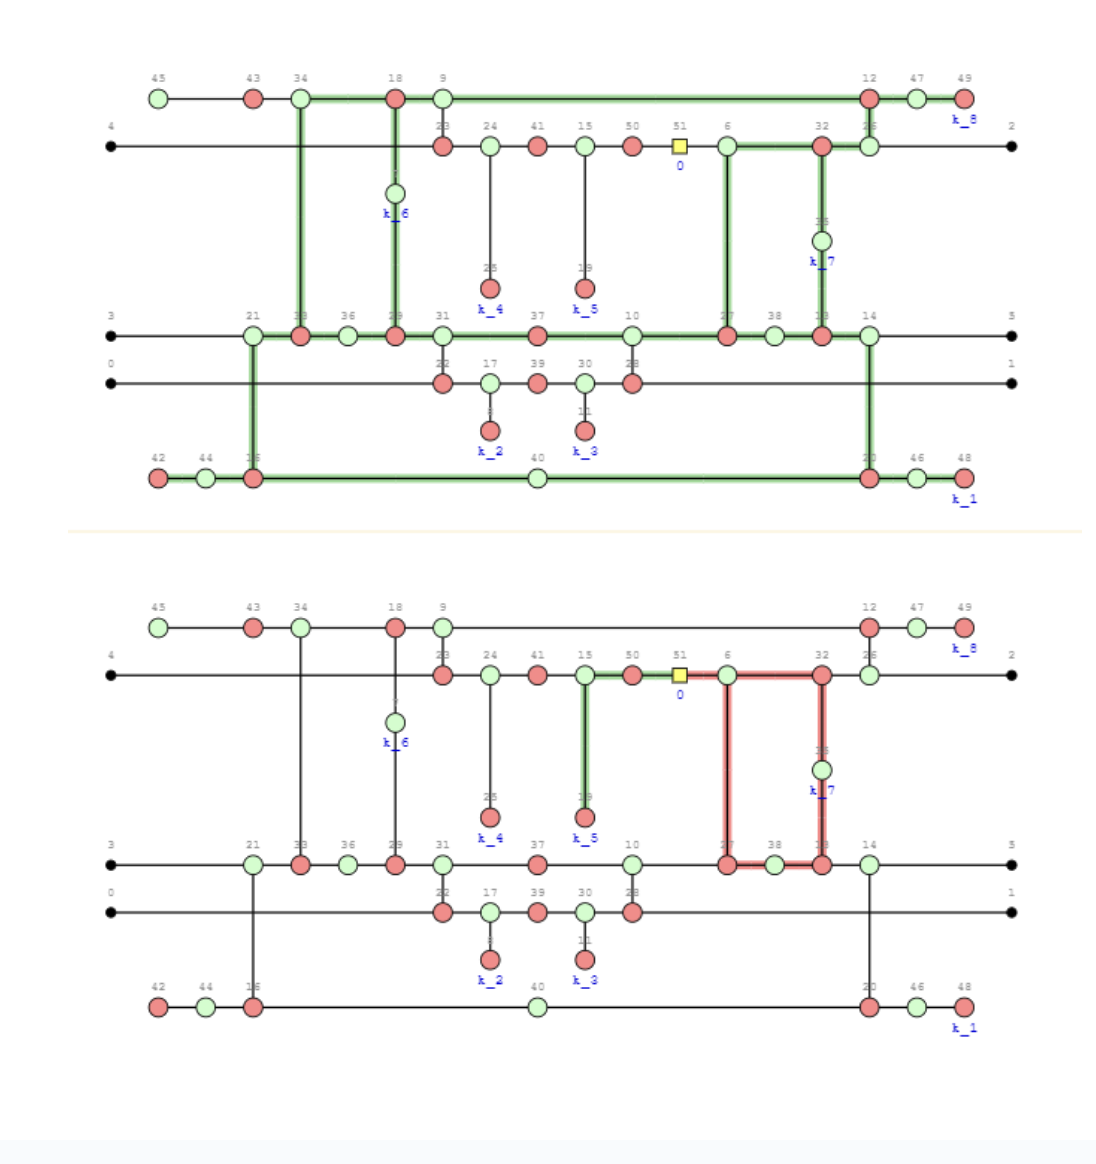
\includegraphics[height=0.7\textheight]{img/xxx_detwebs.png}
                \caption{Rewritten XXX measurements}
            \end{figure}
        \end{column}
    \end{columns}
\end{frame}

\begin{frame}{Example: Steane Code}
    Theoretically, the pure stabilizer measurements of this code involve weight-4 measurements:
    \begin{figure}
        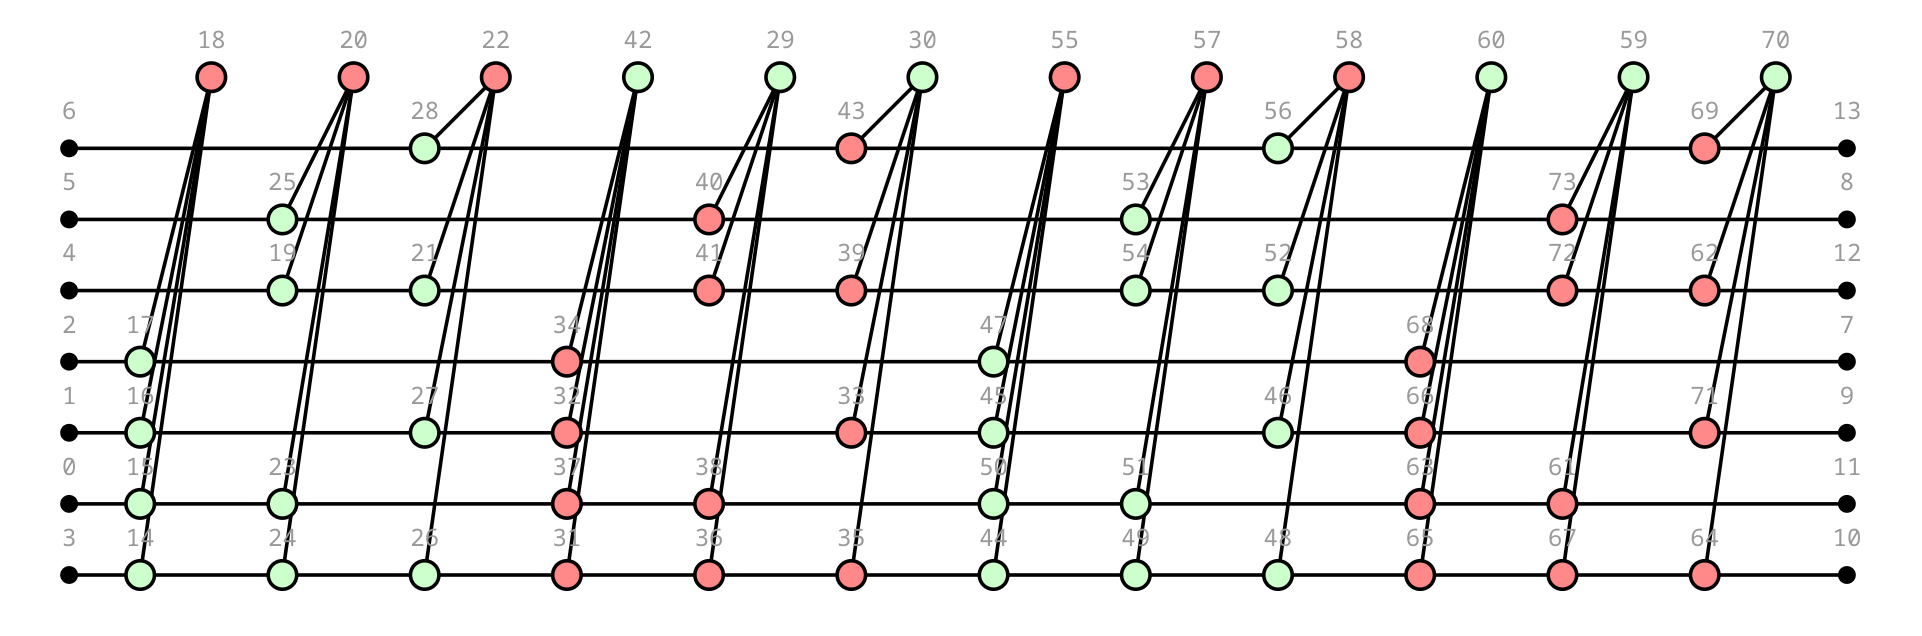
\includegraphics[width=\textwidth]{img/2roundsSteane.png}
        \caption{two rounds of the Steane code stabilizer measurements}
    \end{figure}
\end{frame}
\begin{frame}{Example: Steane Code}
    Theoretically, the pure stabilizer measurements of this code involve weight-4 measurements:
    \begin{figure}
        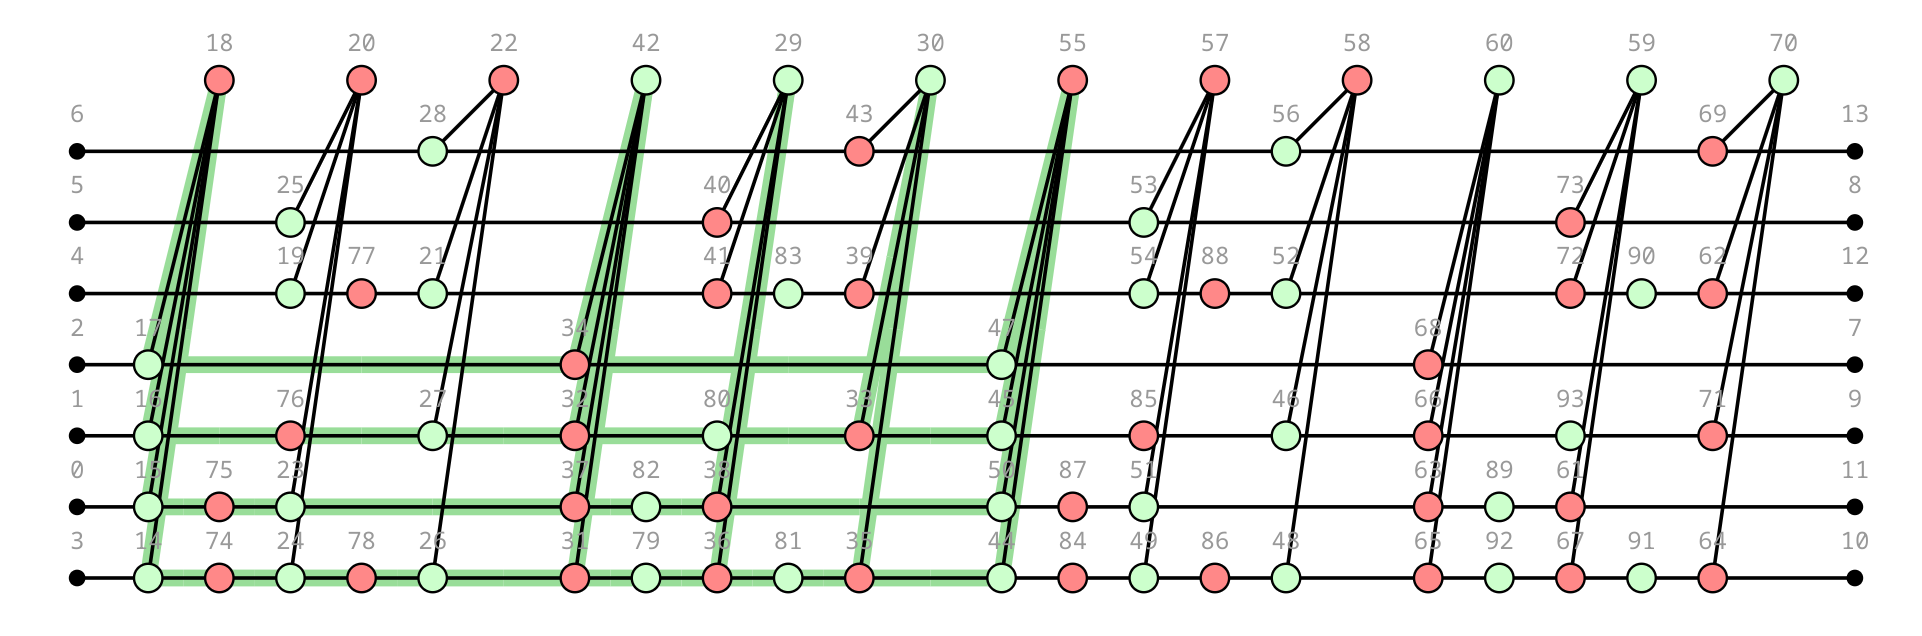
\includegraphics[width=\textwidth]{img/2roundsSteaneDet.png}
        \caption{A detector on the theoretical steane code}
    \end{figure}
\end{frame}

\begin{frame}{Example: Steane Code}
    We can use distance preserving rewrites to get more efficient realisations of previously known
    fault-tolerant syndrome extraction techniques
    \begin{figure}
    \centering
    \begin{subfigure}[t]{0.48\textwidth}
      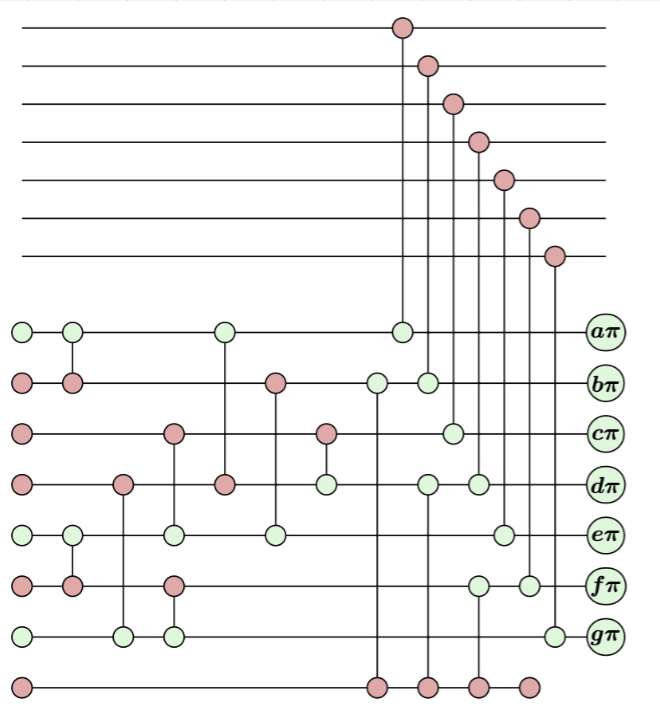
\includegraphics[width=\linewidth]{img/steaneStyleSteaneNormal.png}
      \caption{Steane-Style syndrome extraction}
    \end{subfigure}
    \hfill
    \raisebox{3.6em}{
    \begin{subfigure}[t]{0.48\textwidth}
      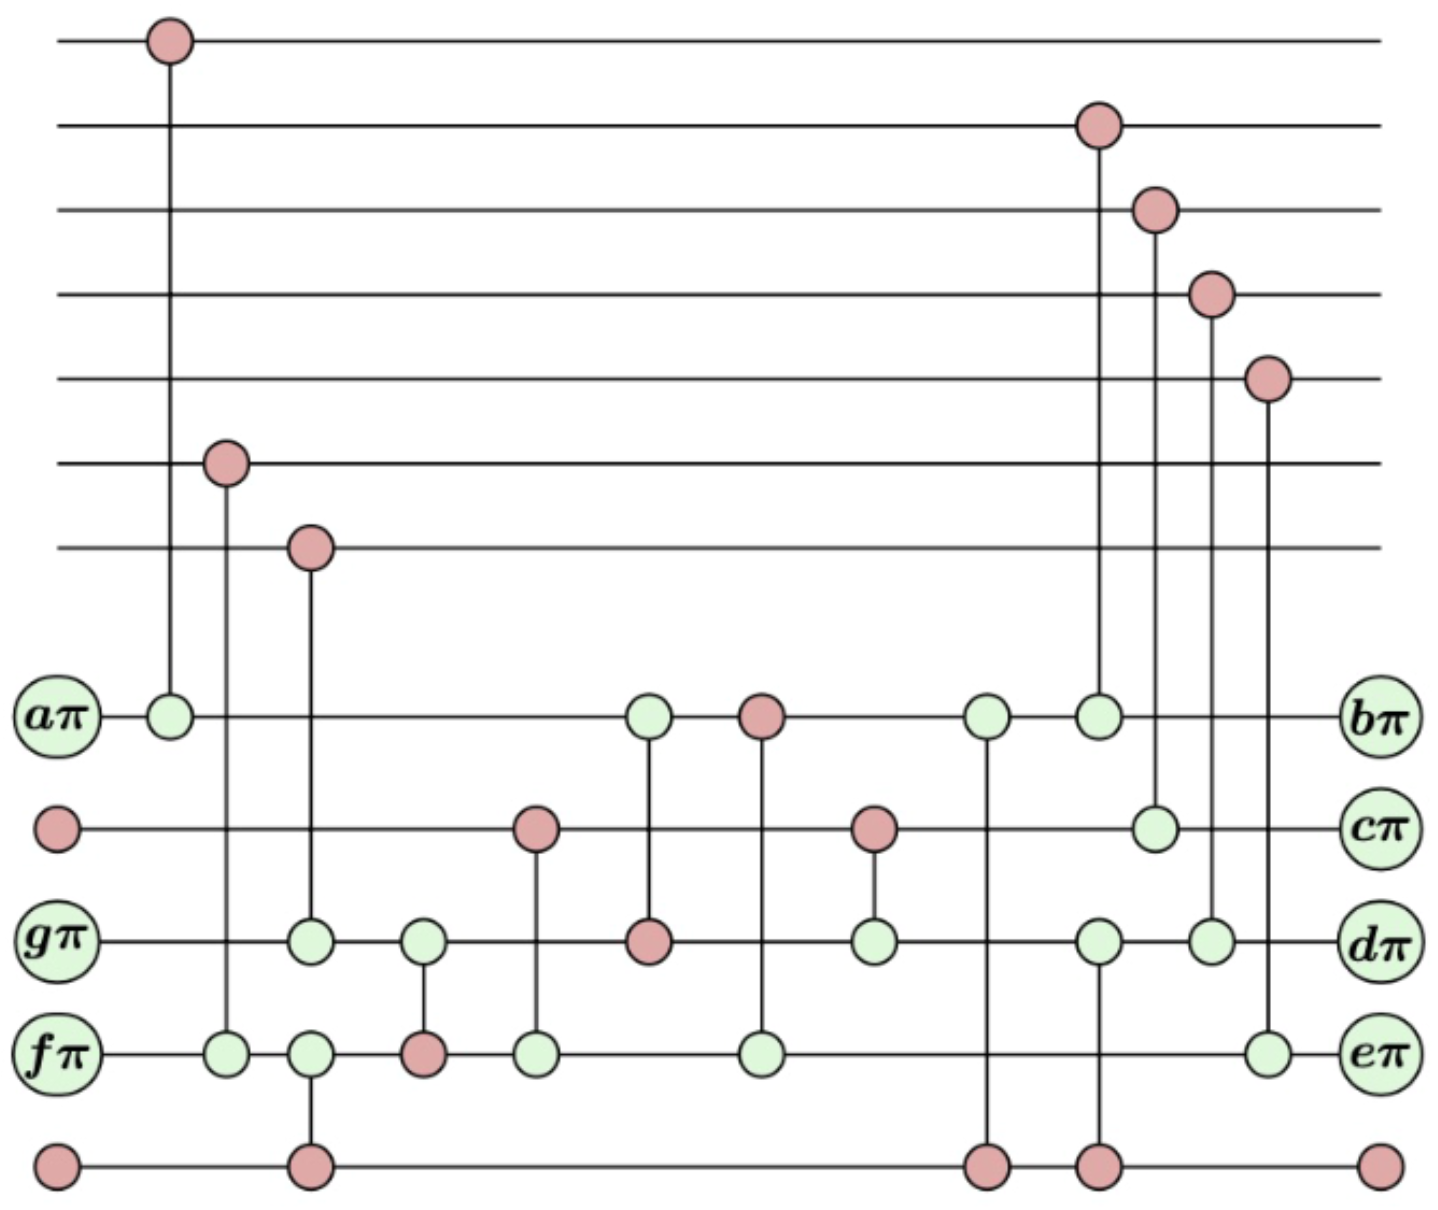
\includegraphics[width=\linewidth]{img/steaneStyleSteaneRewrite.png}
      \caption{Rewrite using fewer ancillas and CNOTs but preserving distance}
    \end{subfigure}
    }
  \end{figure}
\end{frame}



\begin{frame}{Detection webs on rewrite of steane-style Steane measurements}
    \begin{figure}
        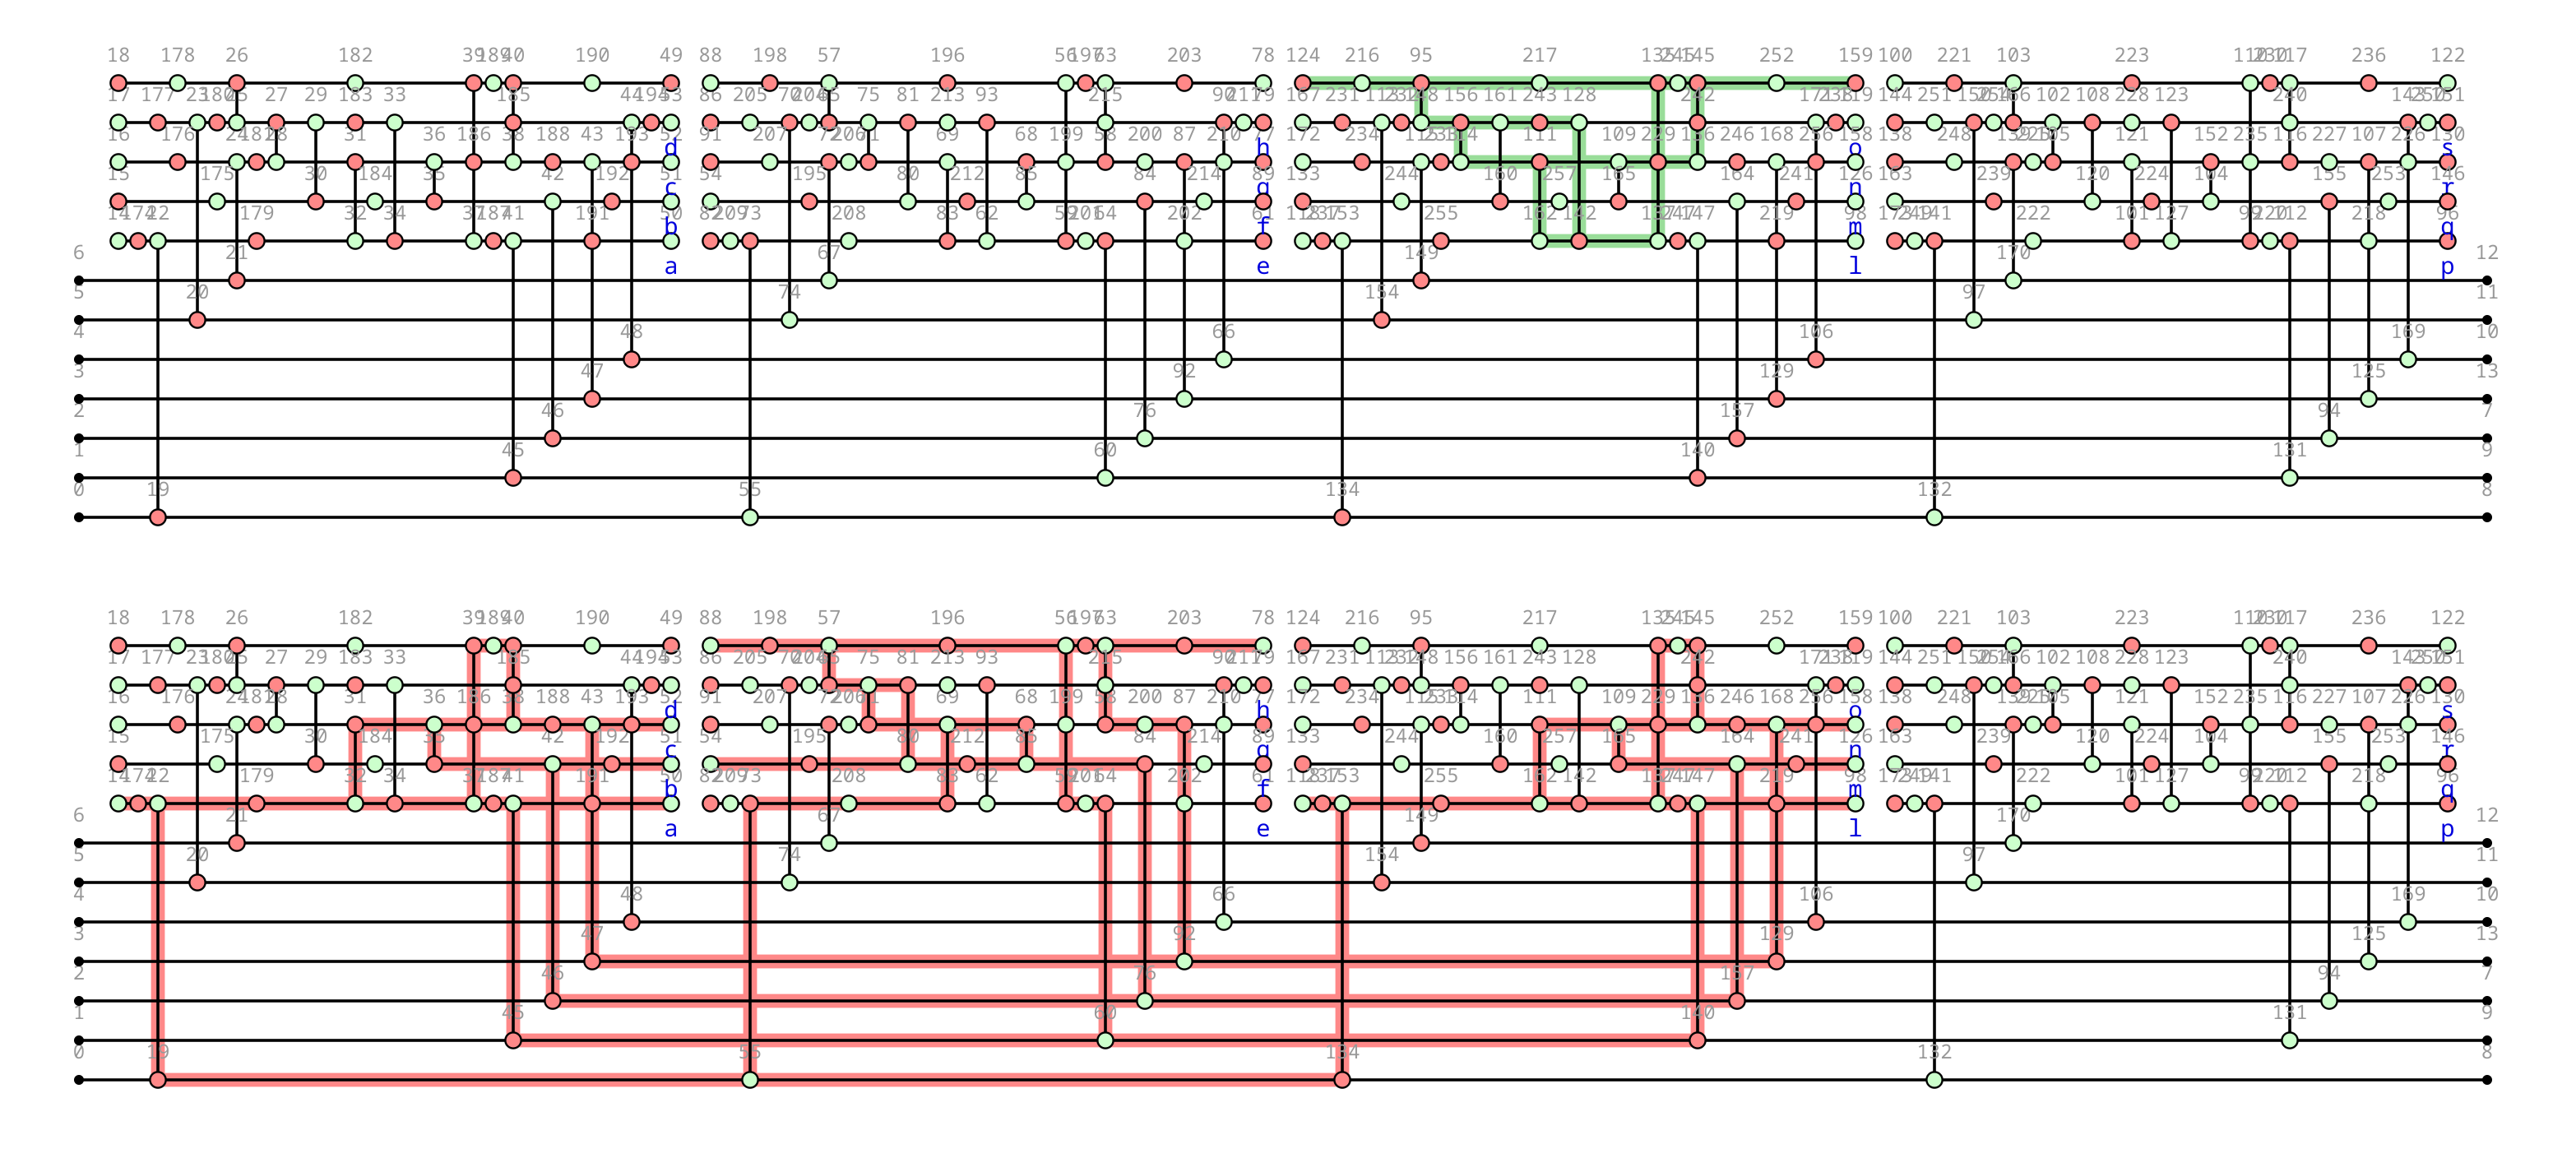
\includegraphics[width=\textwidth]{img/steane_style_steane_webs.png}
        \caption{Rewritten Steane code and two of its detection regions}
    \end{figure}
    
\end{frame}


\section{Outlook}
\begin{frame}
  \centering
  \Huge \insertsection
\end{frame}
\subsection{More general noise models}
\begin{frame}
  \centering
  \Huge \insertsubsection
\end{frame}
\begin{frame}{Error Channels in ZX}
    \begin{itemize}
        \item Since an error channel represents an entanglement to the outside world, it is necessarily non-unitary\\
        \hspace{1em} $\Rightarrow$ To represent a nontrivial error channel in ZX we need a good \\
        \hspace{2.5em} way to represent sums of diagrams
        \item The W spider is a useful adition to represent these concisely
    \end{itemize} 
    \begin{figure}
        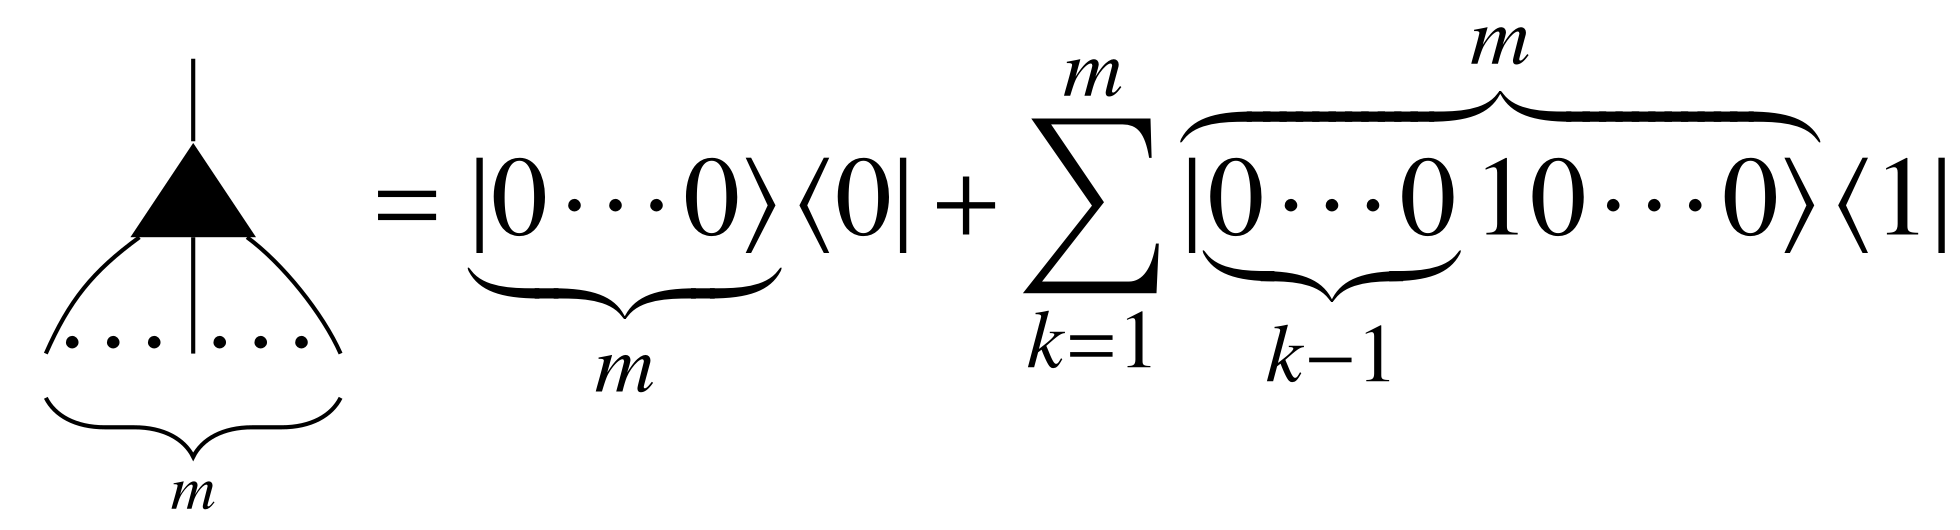
\includegraphics[width=\textwidth]{img/wSpider.png}
        \caption{Definition of W spider}
    \end{figure}
\end{frame}
\begin{frame}{ZXW}
    As a consequence, sums of diagrams become very natural with:
    \begin{figure}
        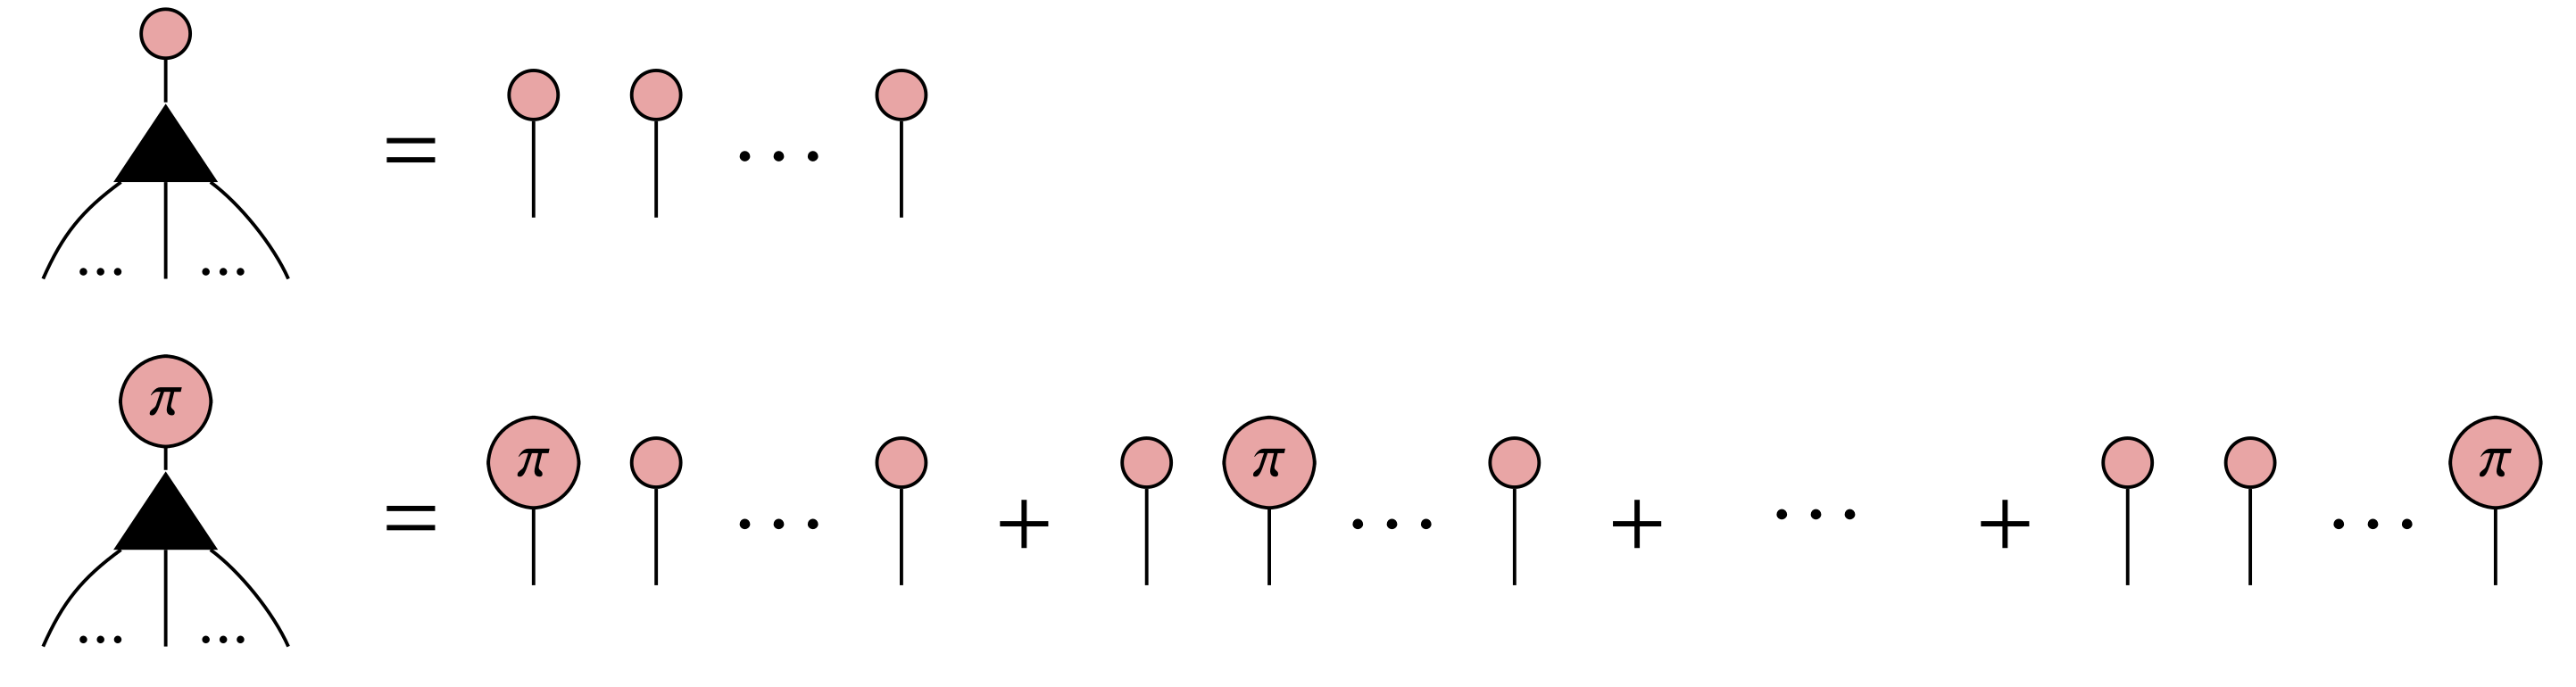
\includegraphics[width=\textwidth]{img/wApplied.png}
        \caption{Effect of W spider with 0 and $\pi$ gadget on diagram.}
    \end{figure}
\end{frame}
\begin{frame}{ZXW}
    \begin{figure}
    \centering
    \begin{subfigure}[t]{0.3\textwidth}
      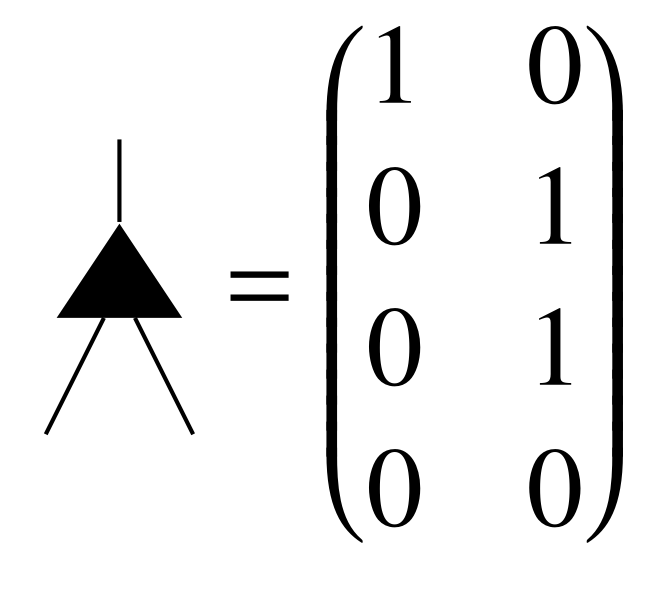
\includegraphics[width=\linewidth]{img/w2spider.png}
      \caption{m=2 W spider}
    \end{subfigure}
    \hfill
    \begin{subfigure}[t]{0.6\textwidth}
      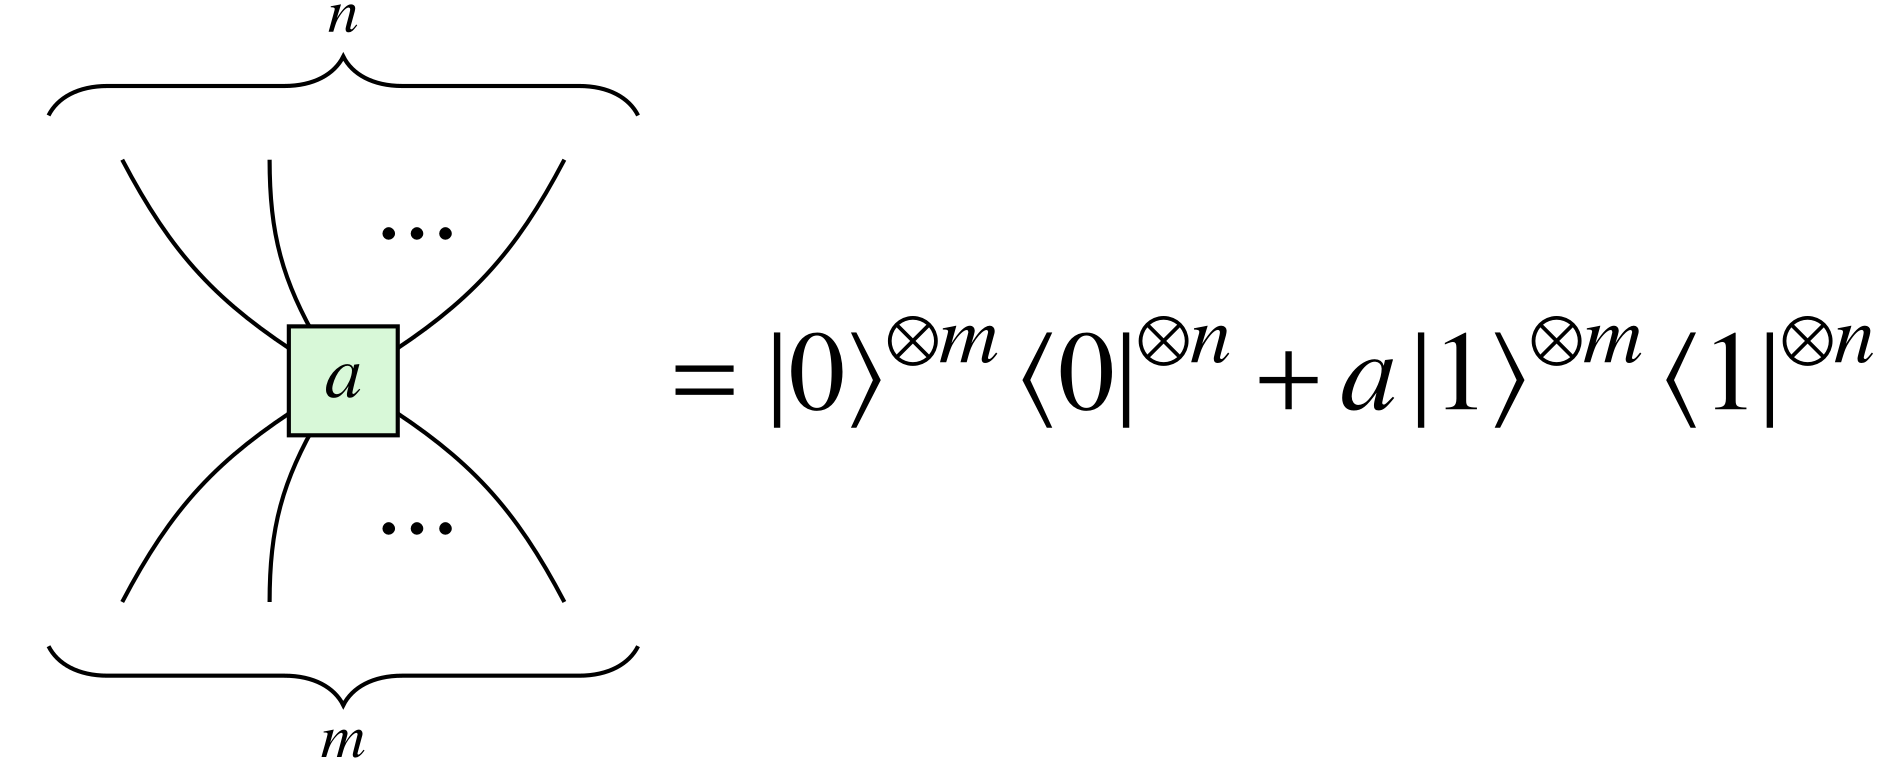
\includegraphics[width=\linewidth]{img/boxspider.png}
      \caption{Box Spider}
    \end{subfigure}
    
    
    
  \end{figure}
\end{frame}
\begin{frame}{ZXW for general hamiltonians}
    Then to represent a hamiltonian of commuting paulis
    $\displaystyle\mathcal{H} = \sum_{i=1}^{n} \alpha_i \bigotimes_{j=1}^m P_{ij}$
    \begin{figure}
        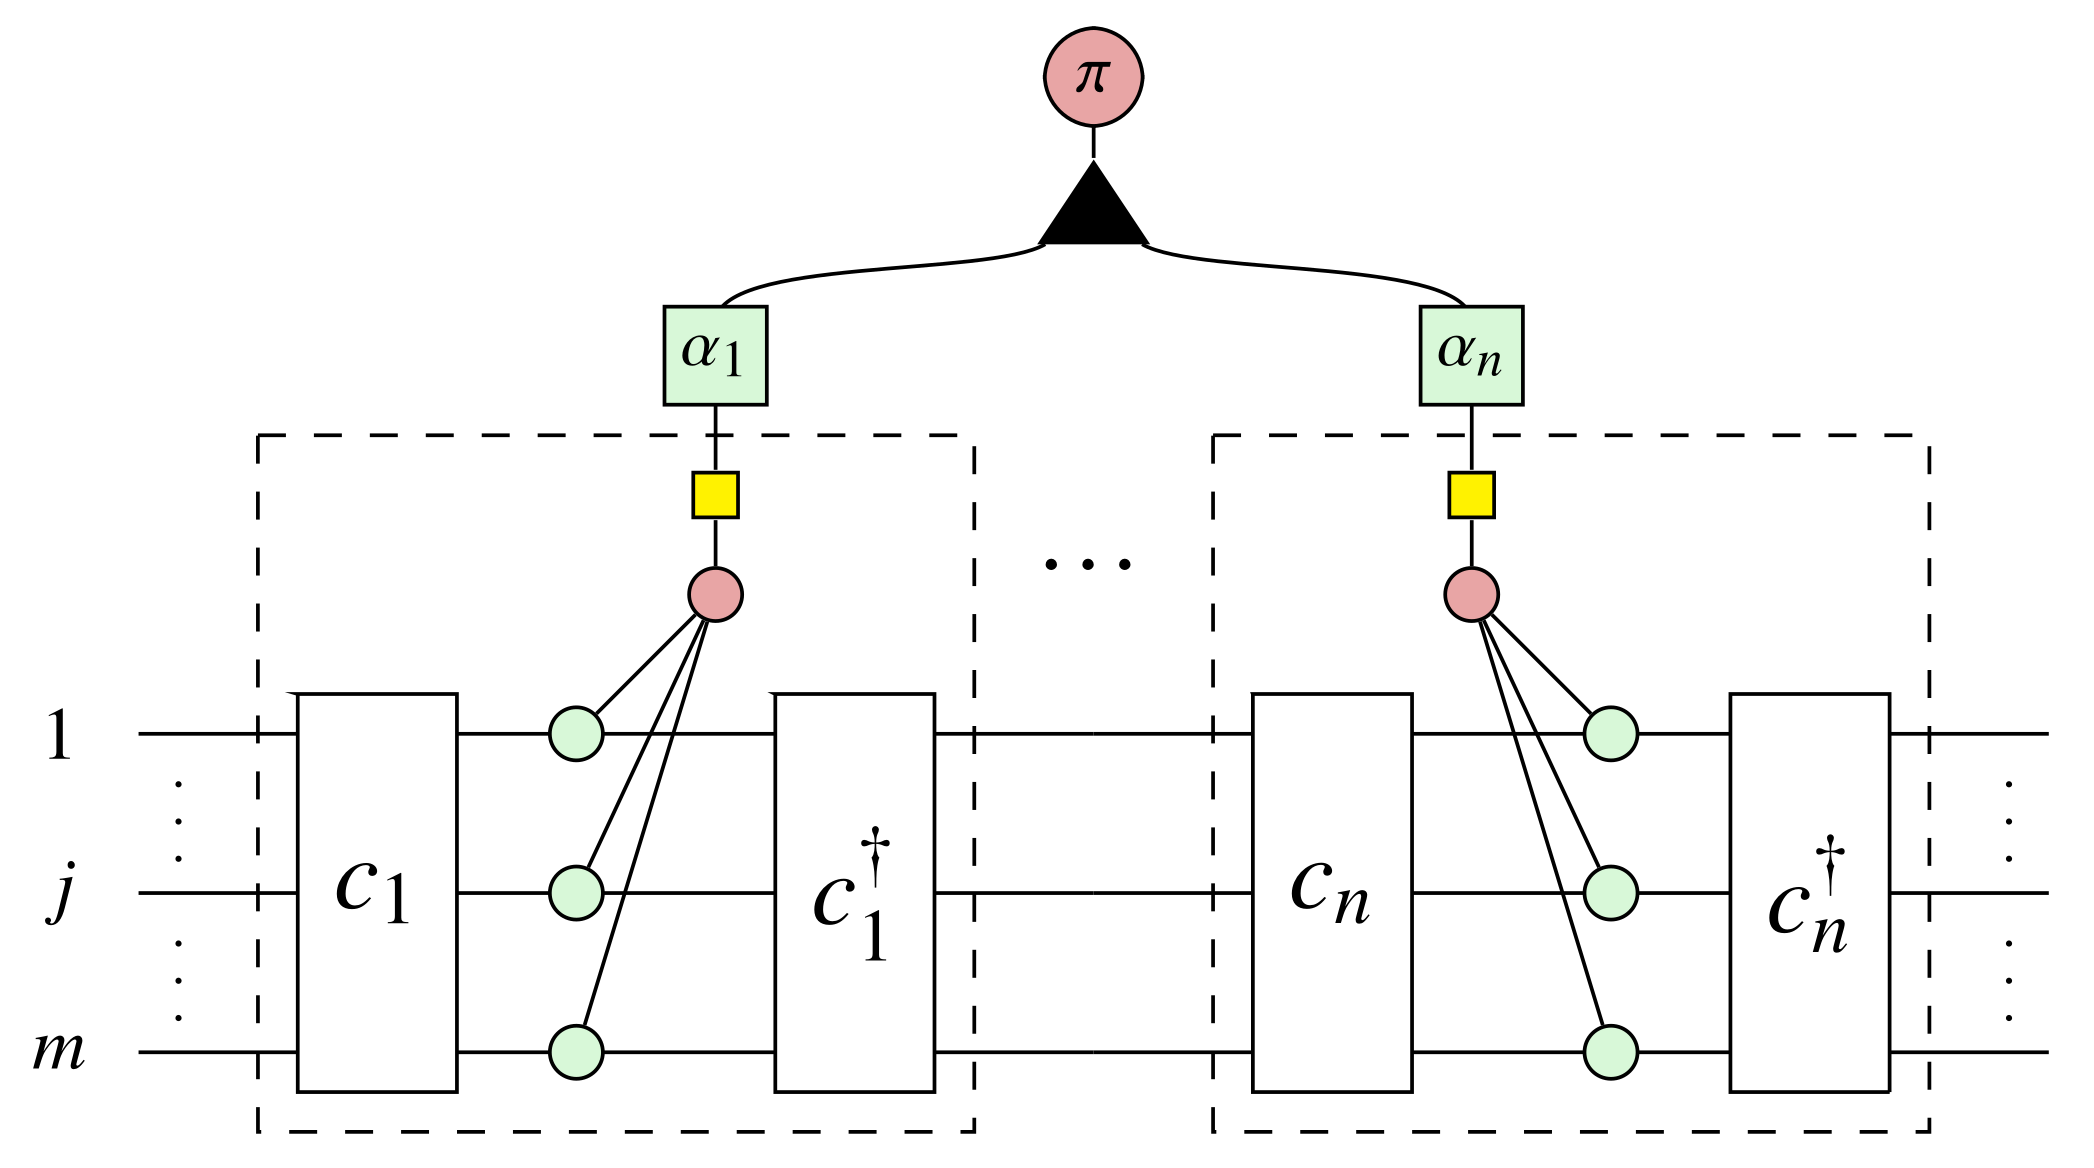
\includegraphics[height=0.6\textheight]{img/sumofdiag.png} 
        \caption{One way to represent a general hamiltonian in ZX. \
        Here $c_{ij}$ are the clifford conjugations of $Z$ to $P_{ij}$}
    \end{figure}
\end{frame}
\subsection{A path to computing thresholds}
\begin{frame}
  \centering
  \Huge \insertsubsection
\end{frame}
\subsubsection{Fidelity in ZX}
\begin{frame}
  \centering
  \Huge \insertsubsubsection
\end{frame}
\begin{frame}{Hilbert-Schmidt fidelity in ZX}
    % \begin{figure}
    %     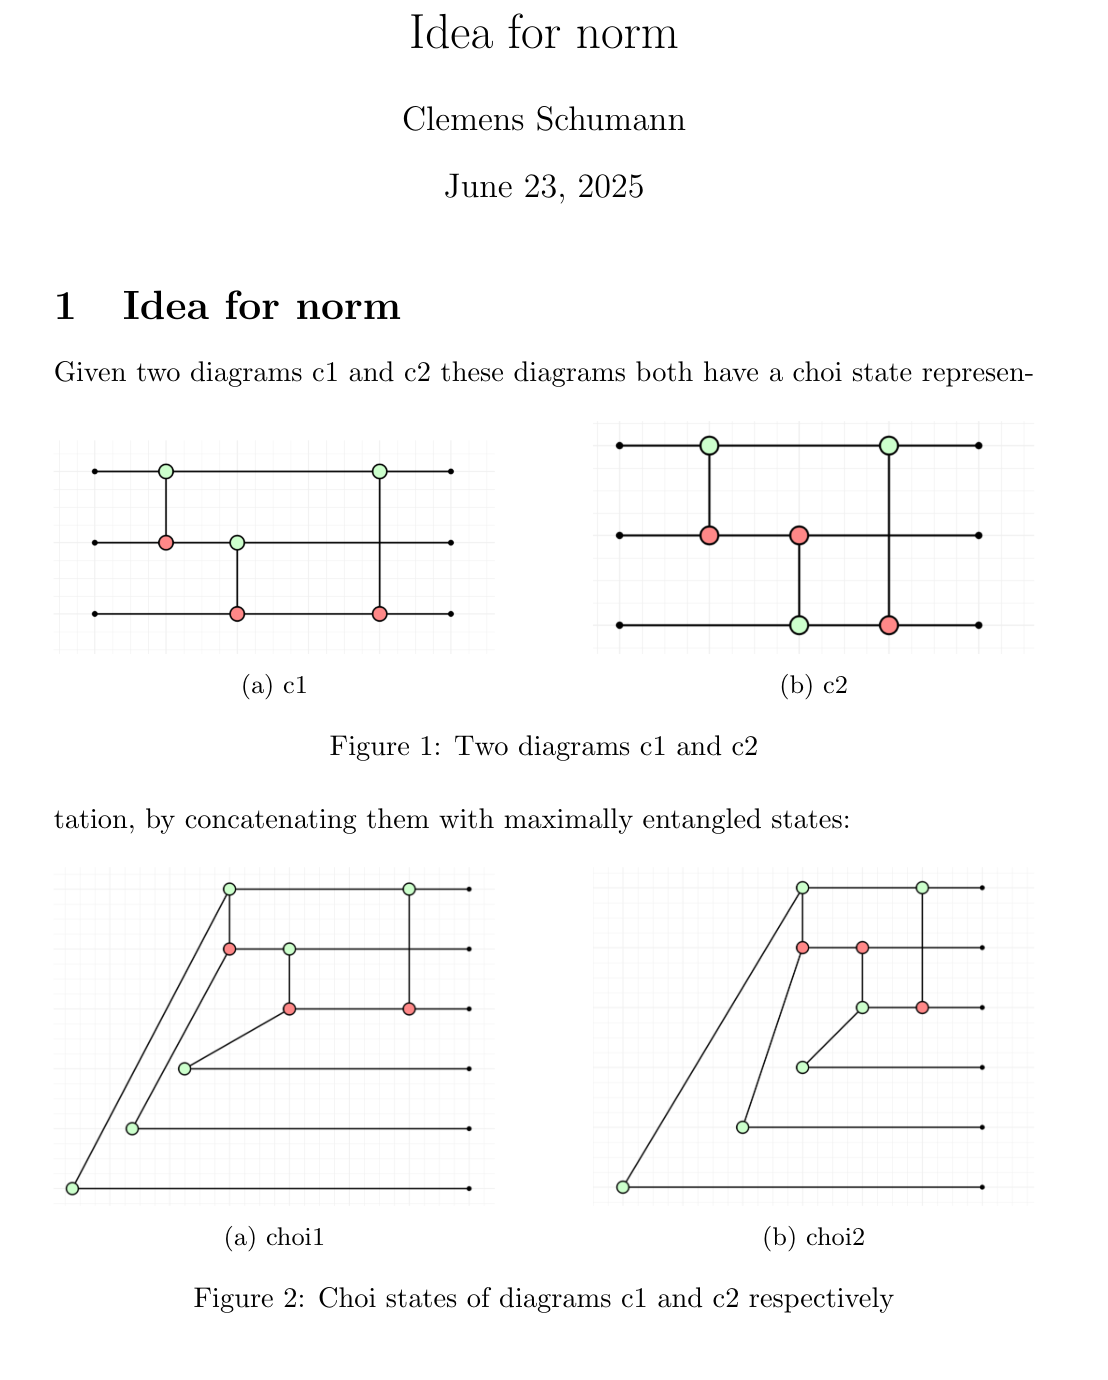
\includegraphics[height=0.7\textheight]{img/fidelity1.png}
    % \end{figure}
    \begin{figure}[htbp]
        \centering
        \begin{subfigure}[b]{0.45\textwidth}
            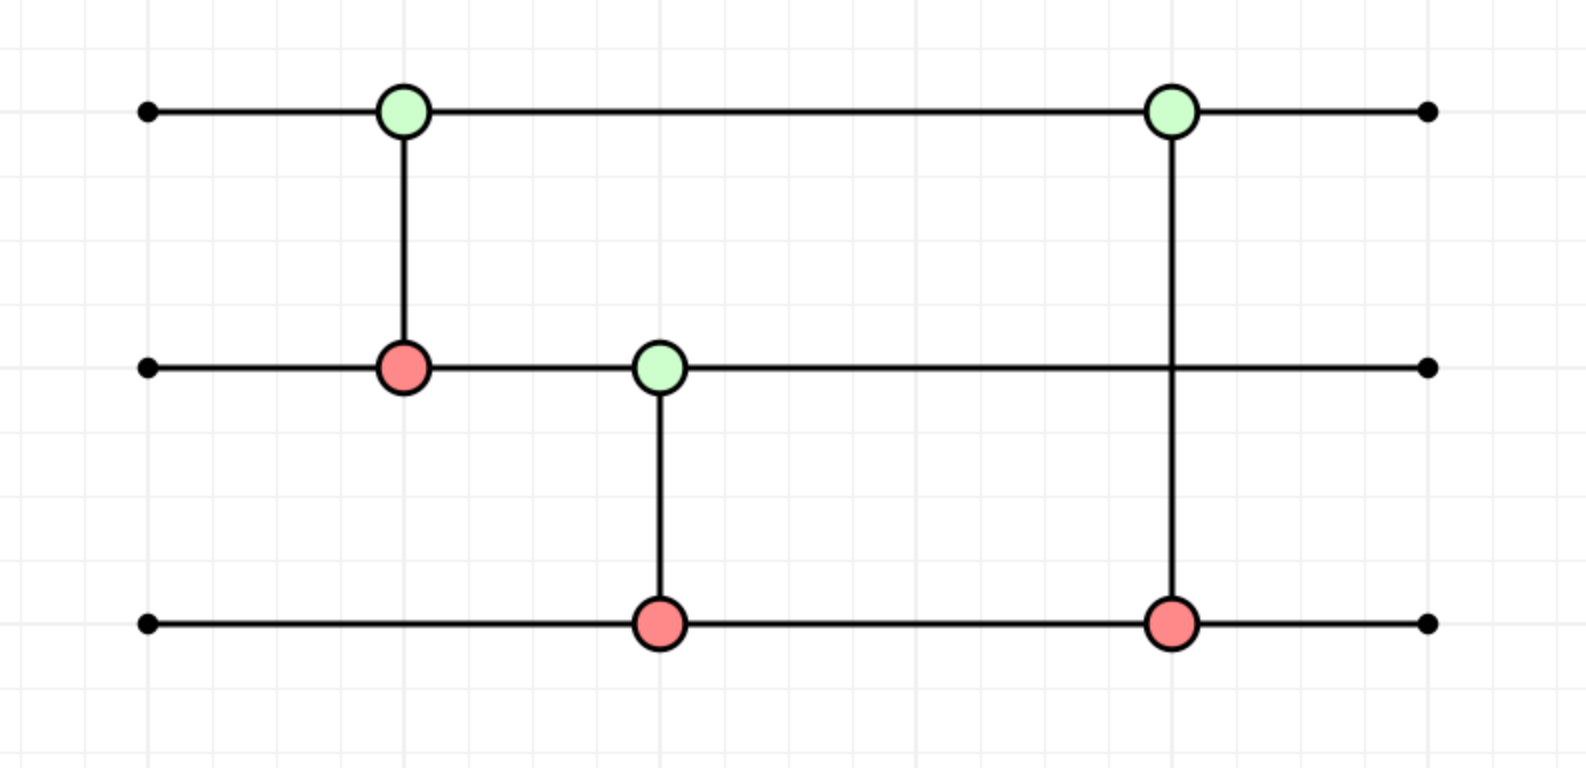
\includegraphics[width=\textwidth]{img/circ1.png}
            \caption{c1}
            \label{fig:subc1}
        \end{subfigure}
    \hfill
    \begin{subfigure}[b]{0.45\textwidth}
        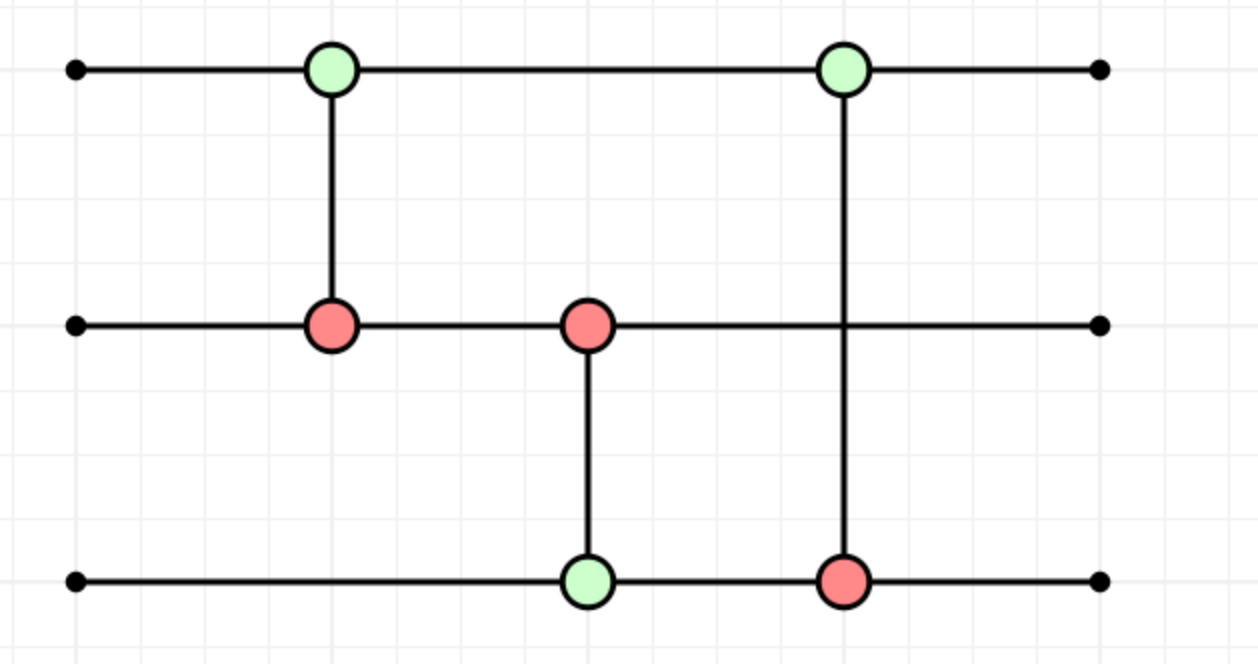
\includegraphics[width=\textwidth]{img/circ2.png}
        \caption{c2}
        \label{fig:subc2}
    \end{subfigure}
    \caption{Two diagrams c1 and c2}
    \label{fig:mainc}
    \end{figure}
\end{frame}
\begin{frame}{Hilbert-Schmidt fidelity in ZX}
    % \begin{figure}
    %     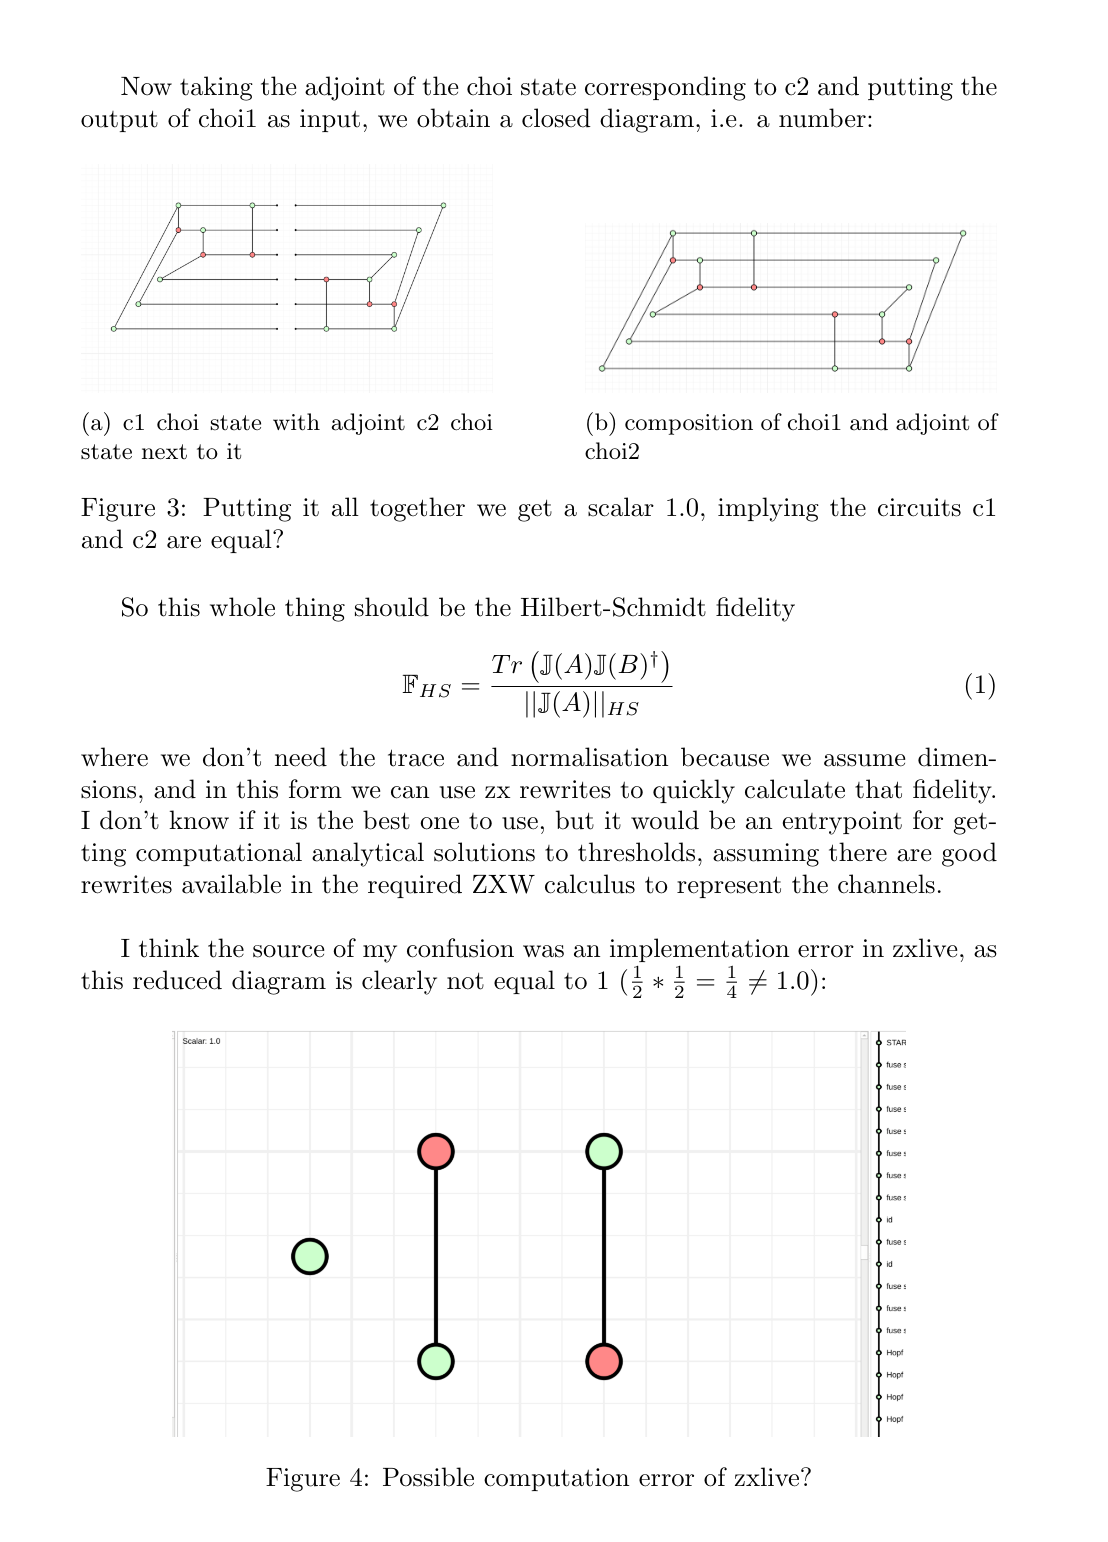
\includegraphics[height=0.7\textheight]{img/fidelity2.png}
    %     \caption{Natuerlich noch aufgeschoenert}
    % \end{figure}
    \begin{figure}[htbp]
    \centering
    \begin{subfigure}[b]{0.45\textwidth}
    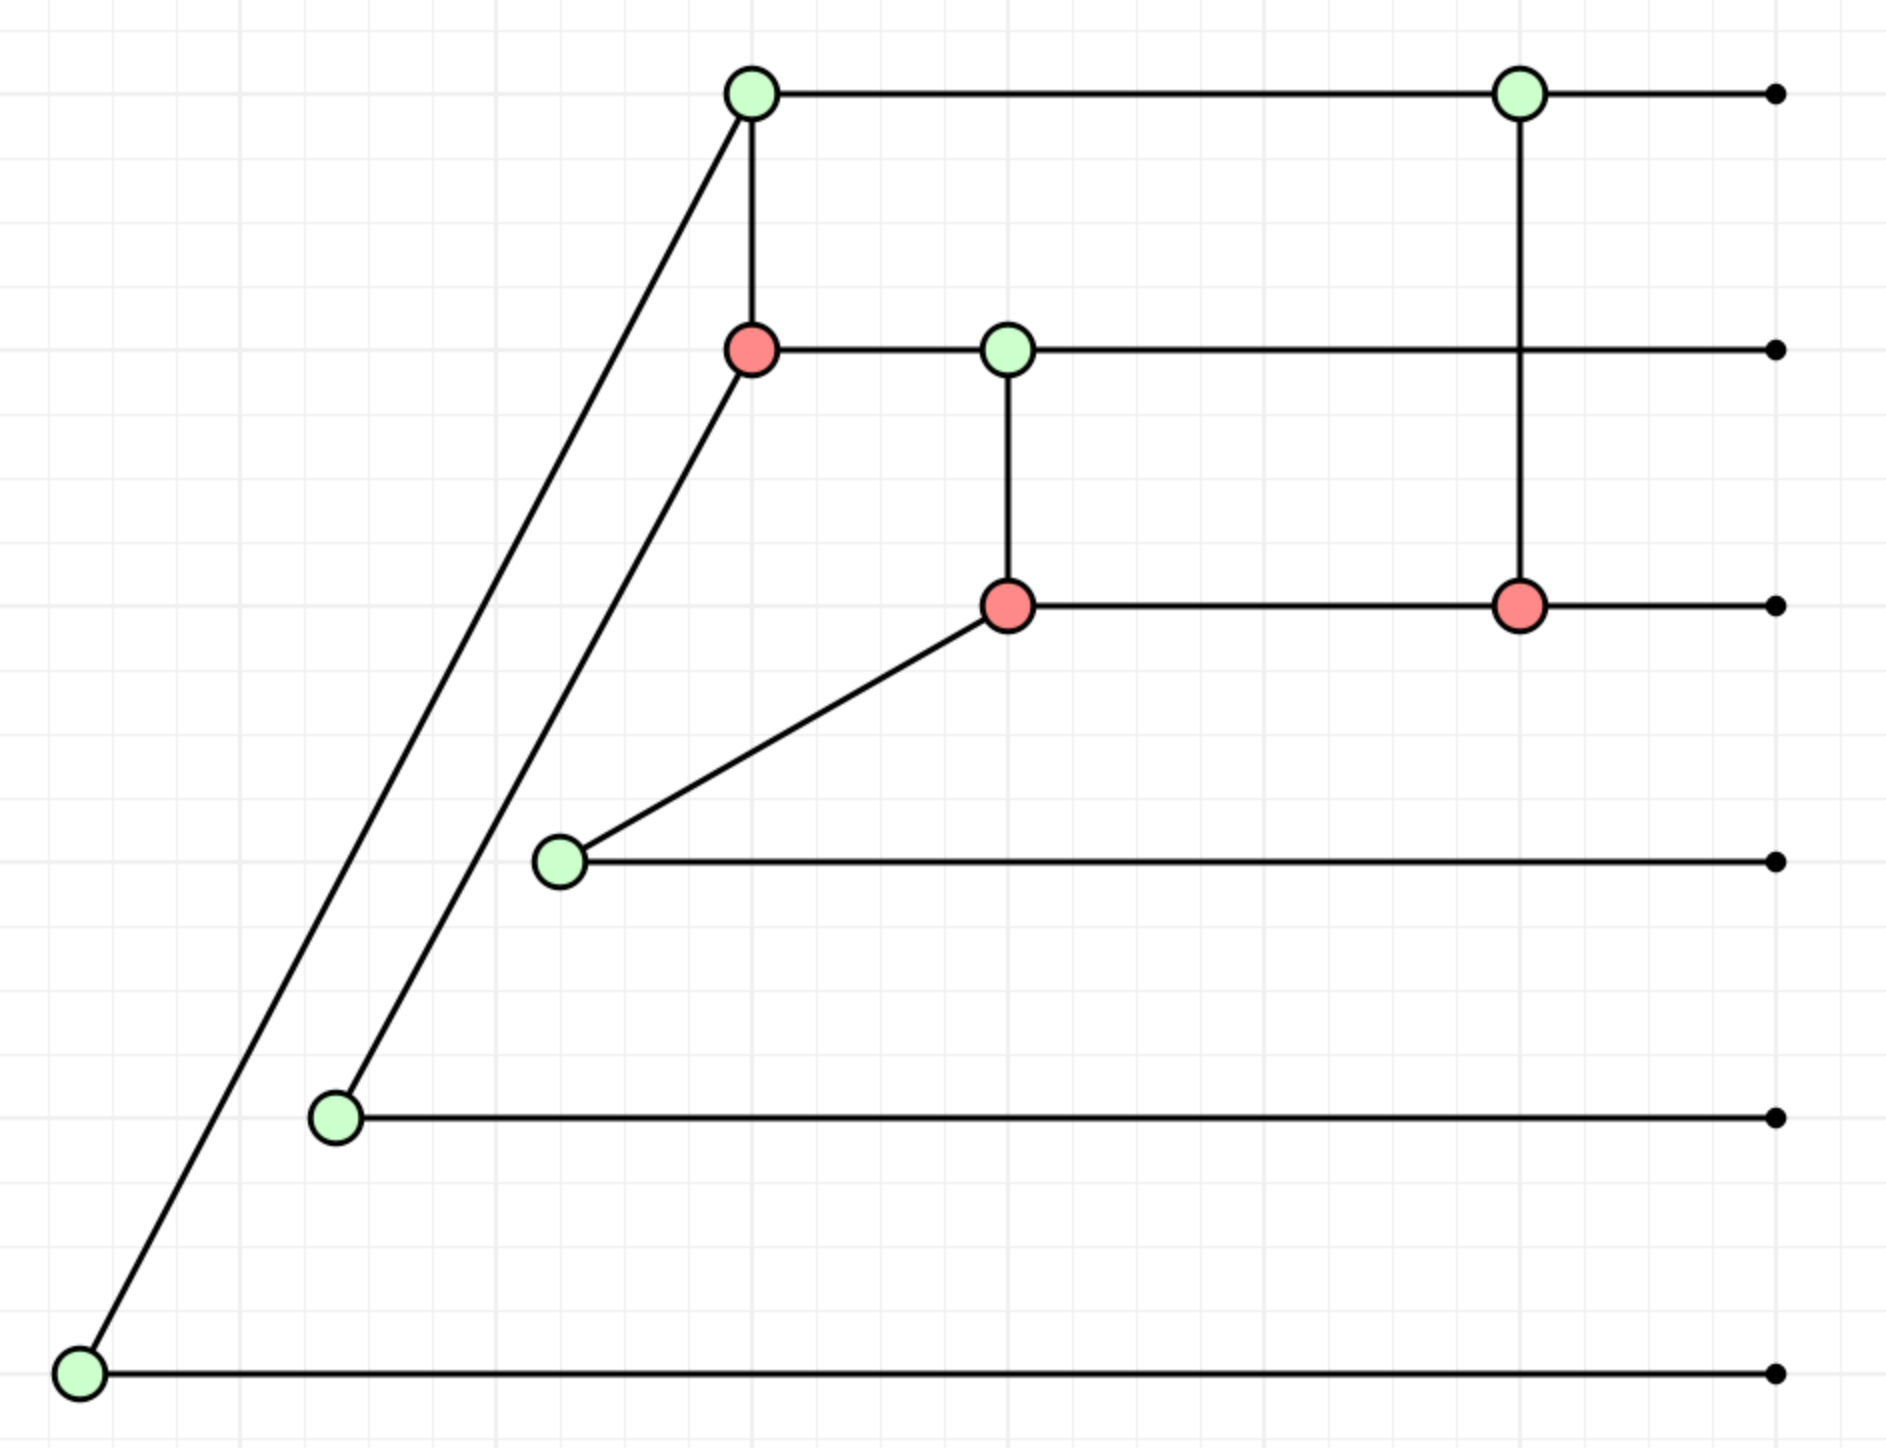
\includegraphics[width=\textwidth]{img/choi1.png}
    \caption{choi1}
    \label{fig:subchoi1}
  \end{subfigure}
  \hfill
  \begin{subfigure}[b]{0.45\textwidth}
    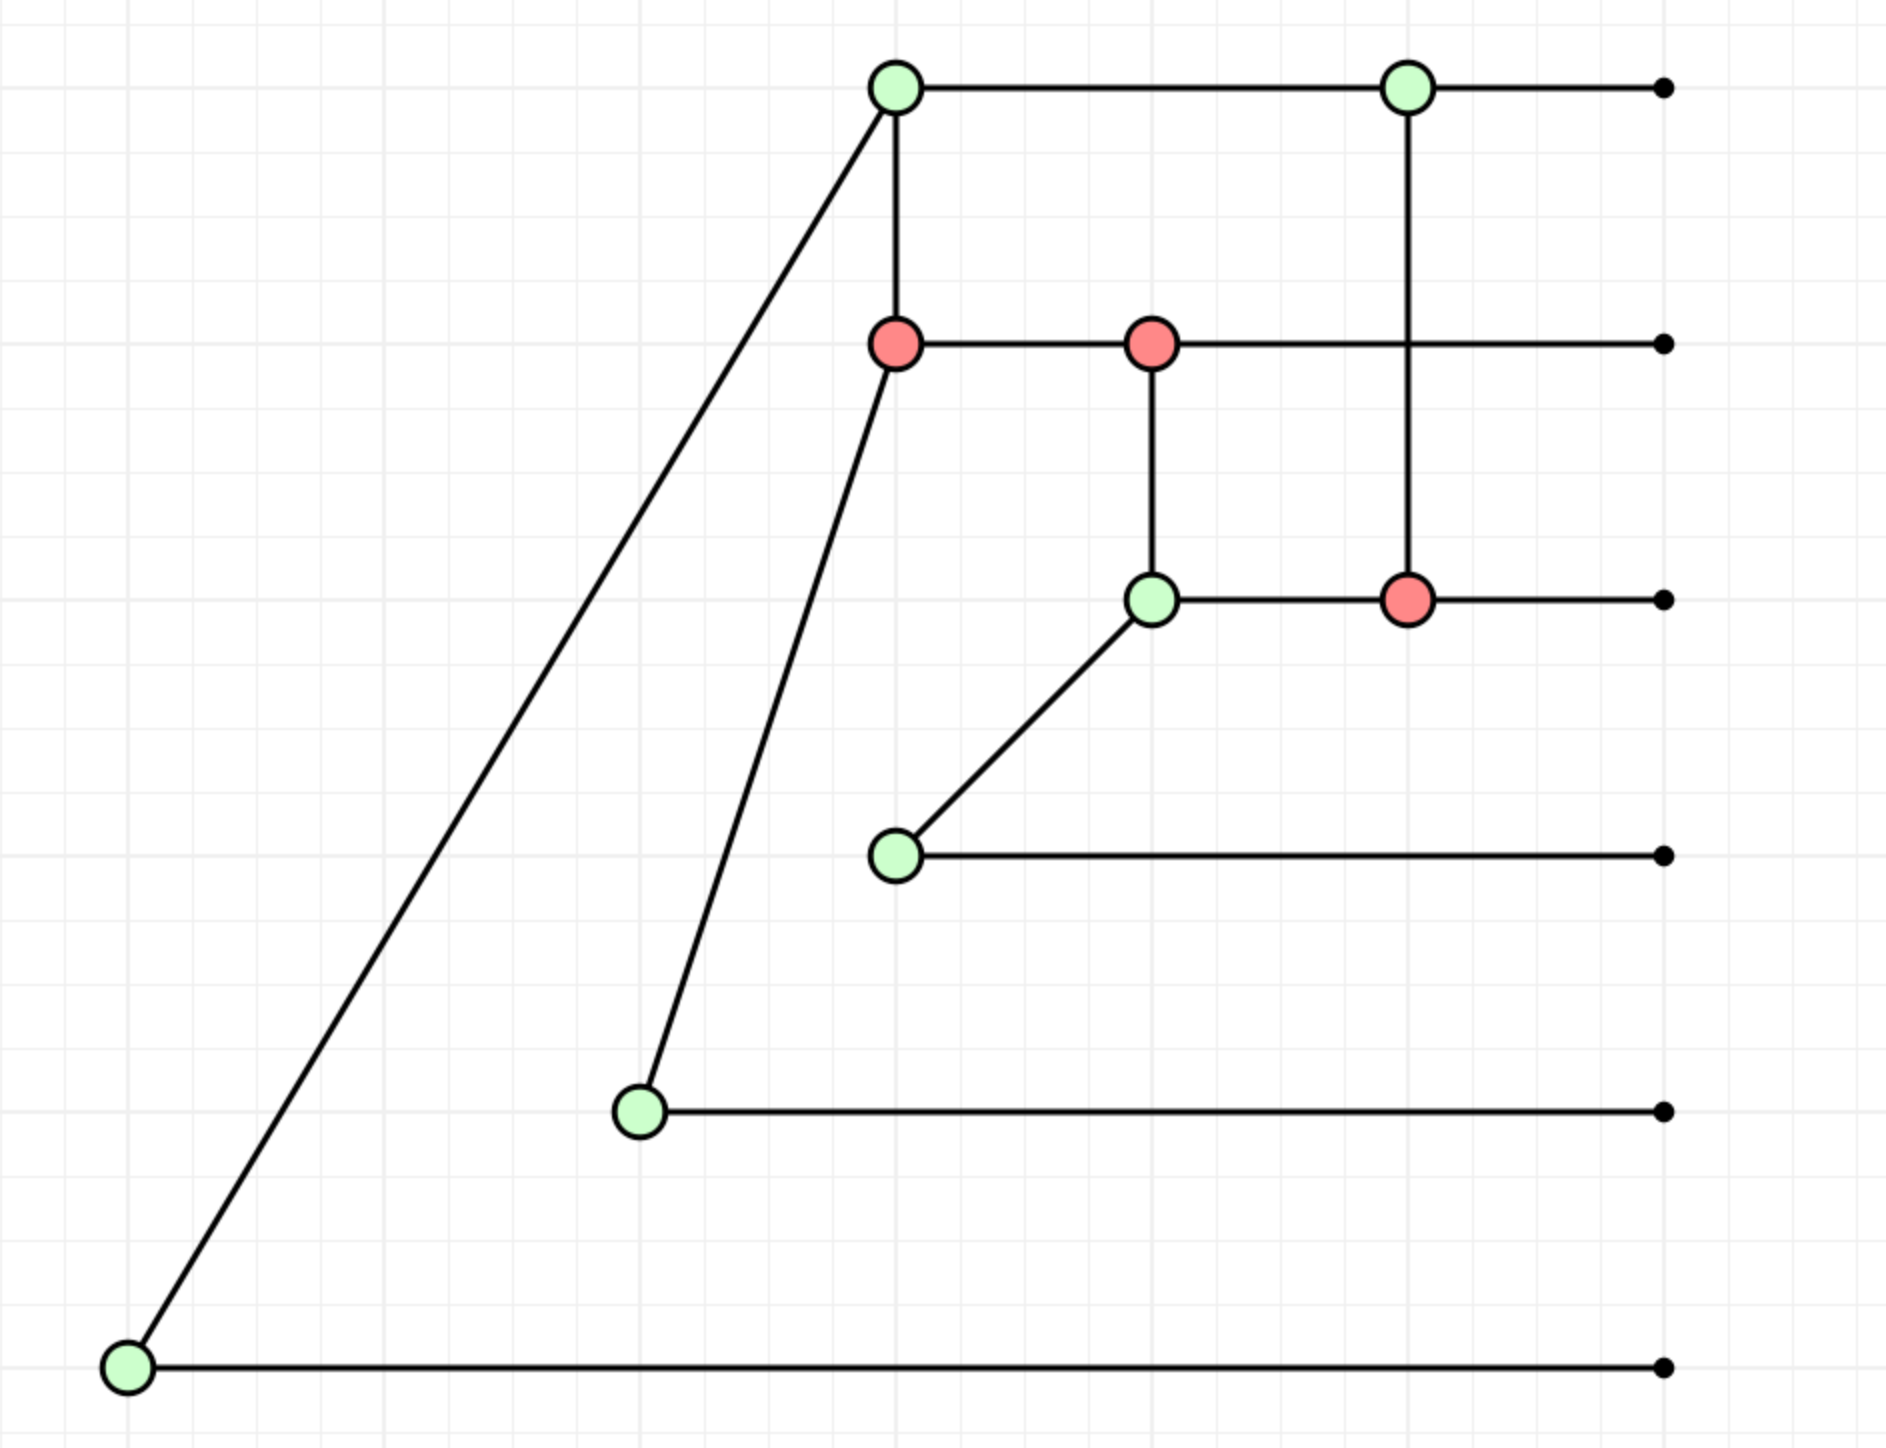
\includegraphics[width=\textwidth]{img/choi2.png}
    \caption{choi2}
    \label{fig:subchoi2}
  \end{subfigure}
  \caption{Choi states of diagrams c1 and c2 respectively}
  \label{fig:mainchoi}
\end{figure}
\end{frame}

\begin{frame}{HS Fidelity}
    Now taking the adjoint of the choi state corresponding to c2
    and putting the output of choi1 as input, we obtain a closed
    diagram, i.e. a number:
    \begin{figure}[htbp]
    \centering
    \begin{subfigure}[b]{0.45\textwidth}
    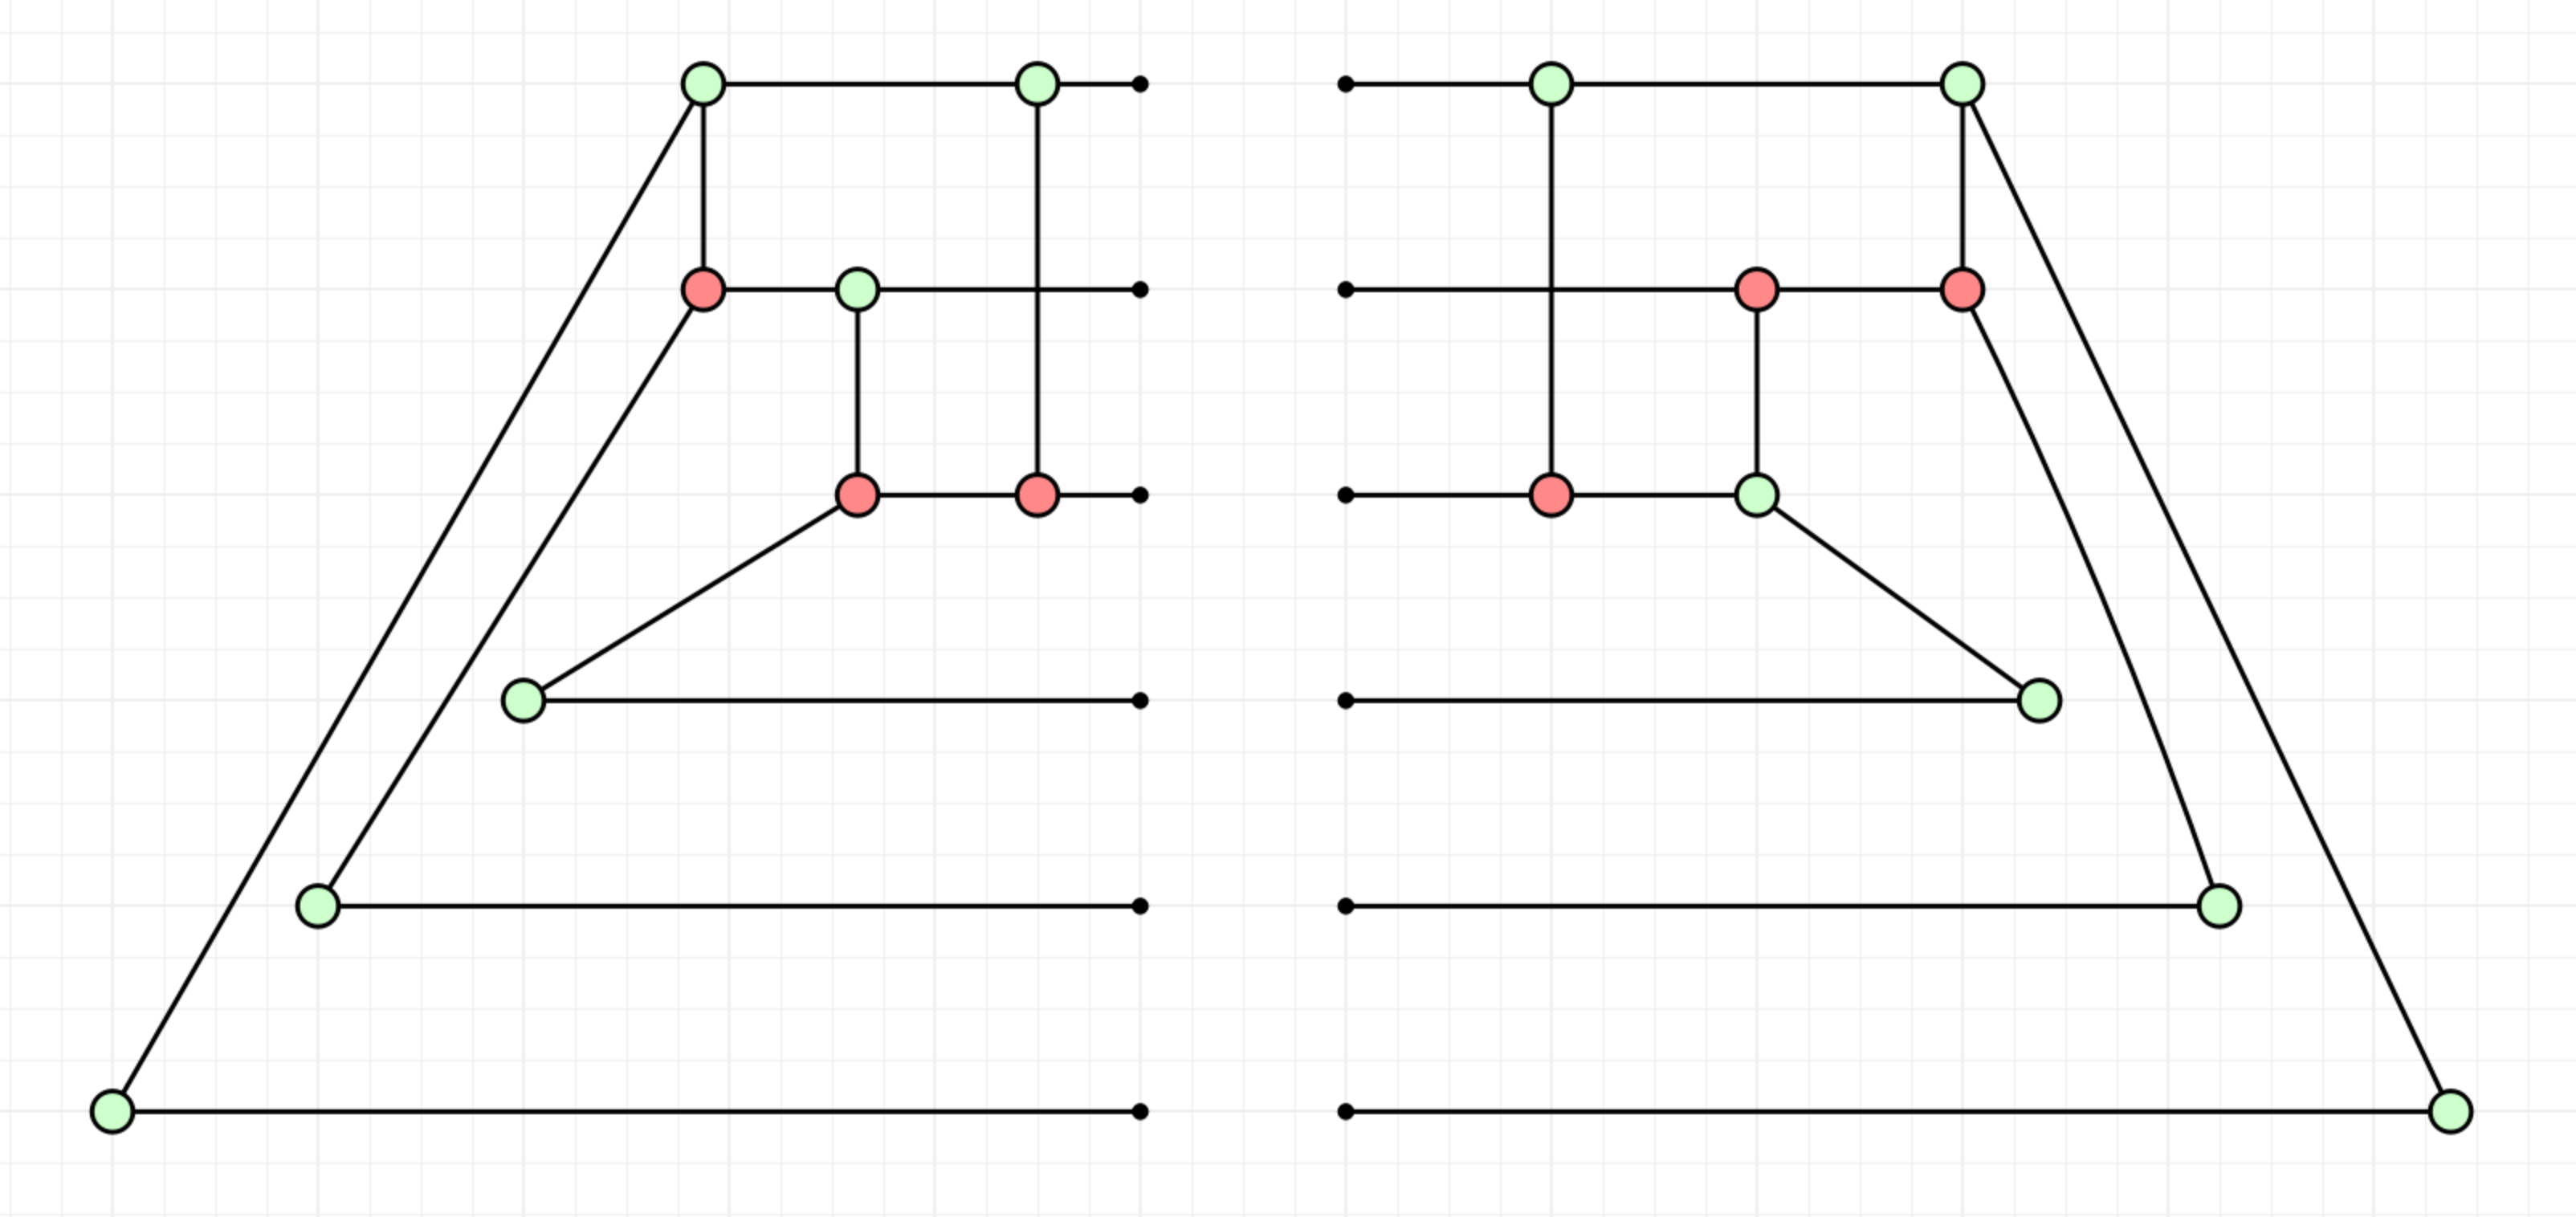
\includegraphics[width=\textwidth]{img/comp1.png}
    \caption{c1 choi state with adjoint c2 choi state next to it}
    \label{fig:comp1}
  \end{subfigure}
  \hfill
  \begin{subfigure}[b]{0.45\textwidth}
    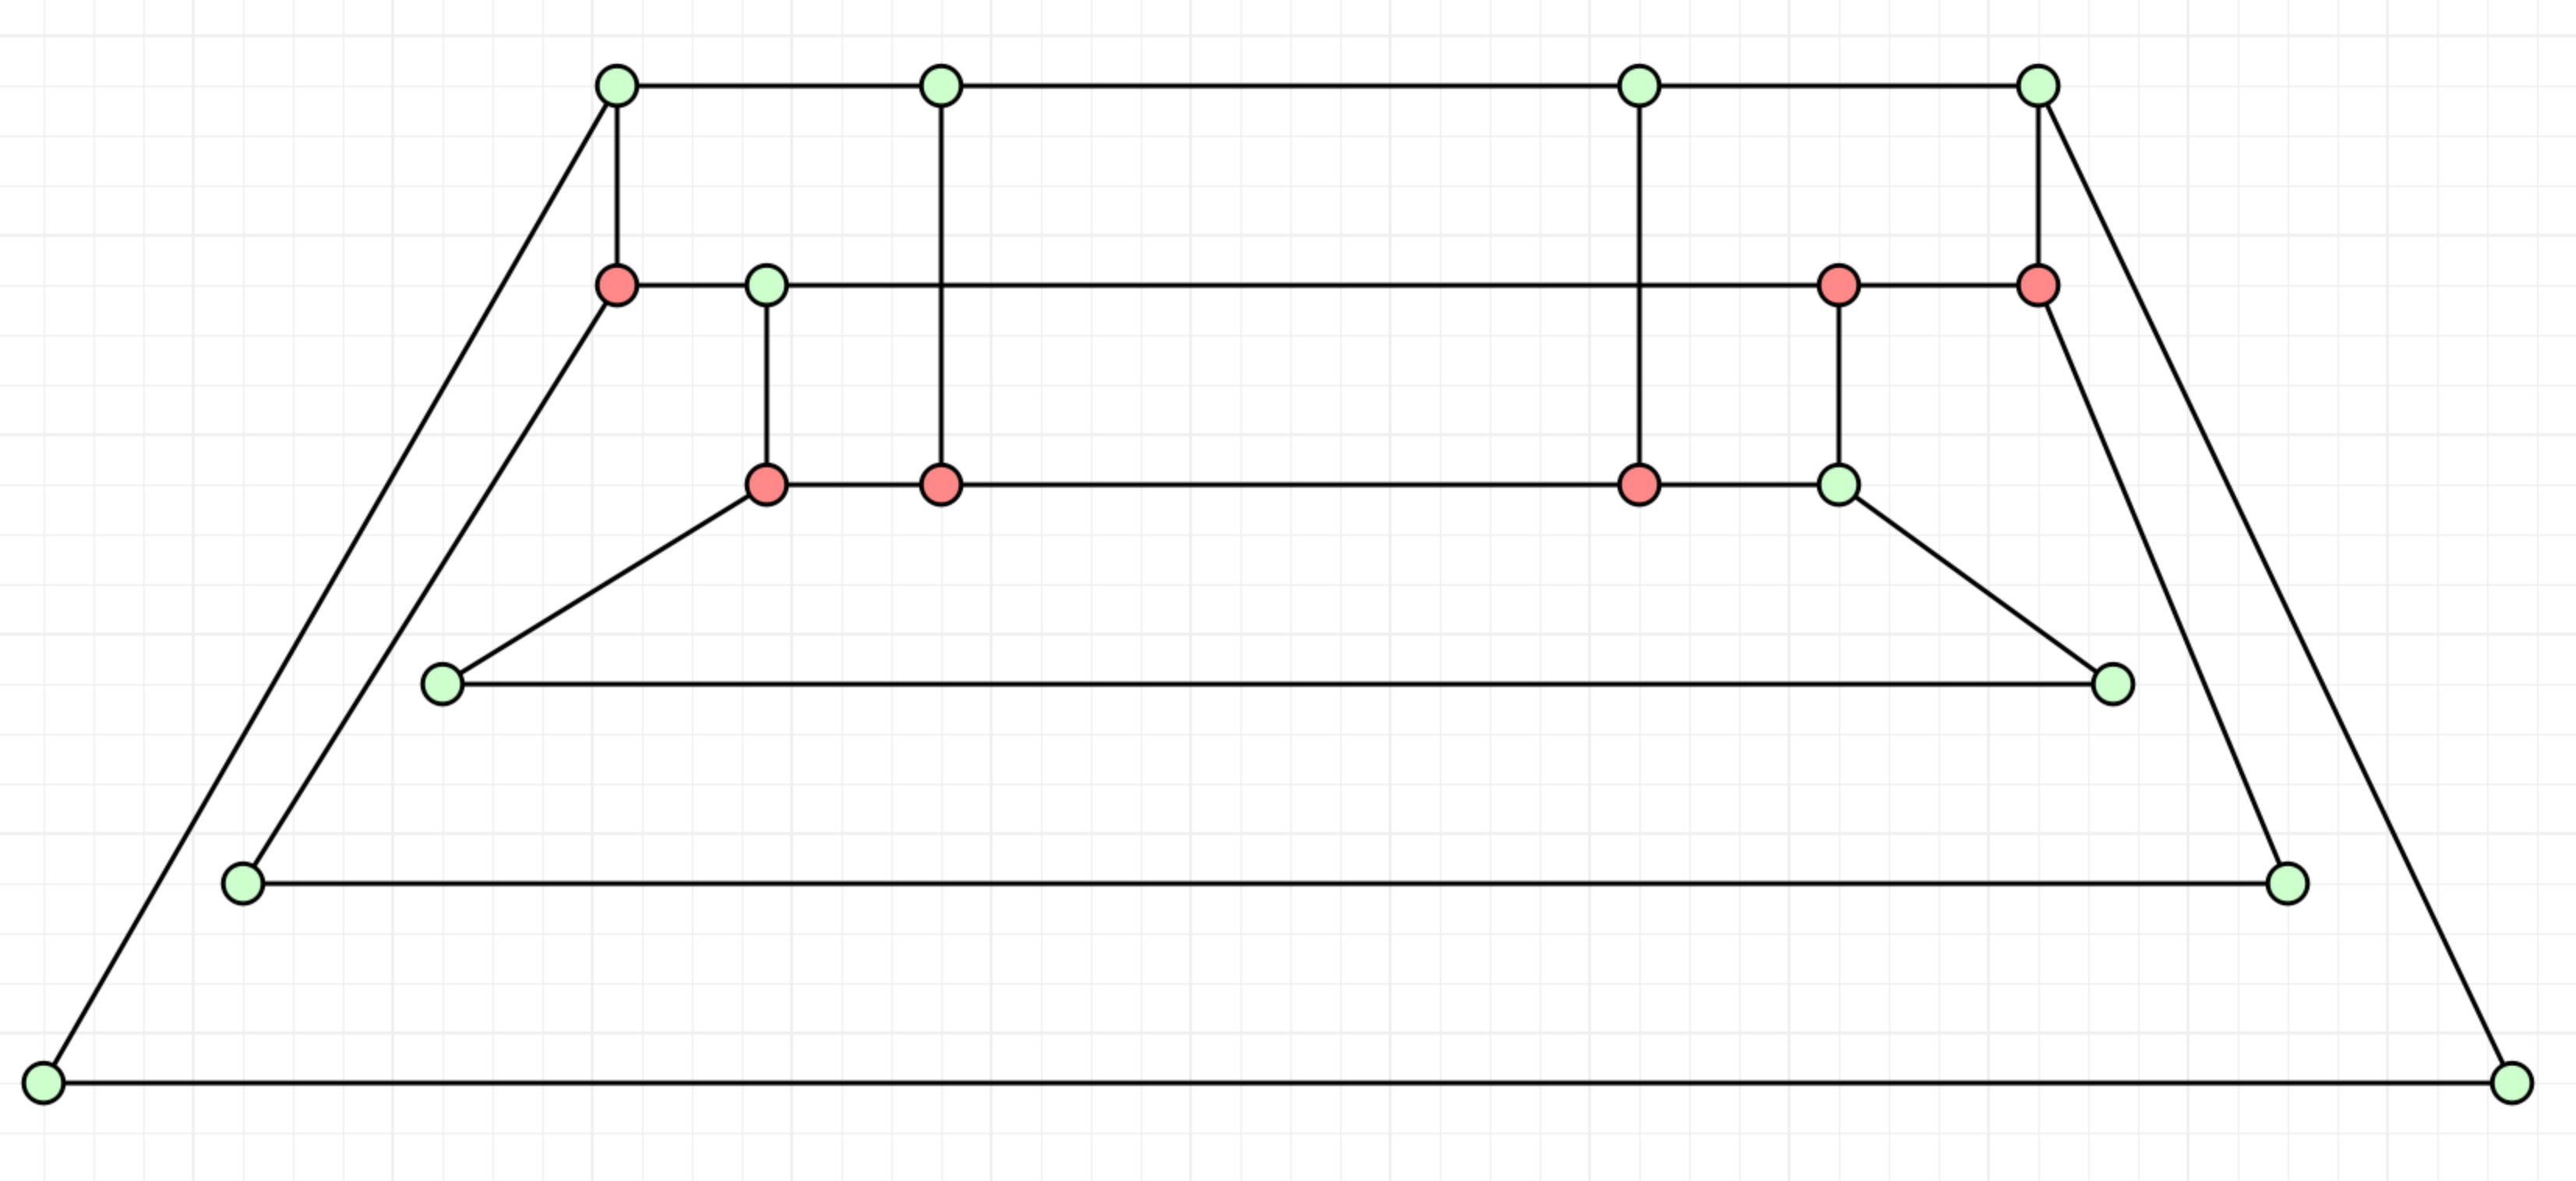
\includegraphics[width=\textwidth]{img/comp2.png}
    \caption{composition of choi1 and adjoint of choi2}
    \label{fig:comp2}
  \end{subfigure}
  \caption{Since this is a closed diagram, it can be simplified to the scalar value $\frac{2}{9}$}
  \label{fig:maincomp}  
\end{figure}
\end{frame}
\begin{frame}{HS Fidelity}
    We can therefore use ZX simplification routines, 
    which reflect symmetries in the map, to \textbf{more efficiently compile fidelity} values.
    The previous example corresponds to the \textbf{Hilbert-Schmidt Fidelity}
    \begin{equation}
        \mathbb{F}_{HS} = \frac{Tr\left( \mathbb{J}(A)\mathbb{J}(B)^{\dagger}\right)}{||\mathbb{J}(A)||_{HS}} 
    \end{equation}
    
\end{frame}

\subsubsection{scalable ZX for reasoning about scalable codes}
\begin{frame}
  \centering
  \Huge \insertsubsubsection
\end{frame}

\begin{frame}
    \begin{figure}
        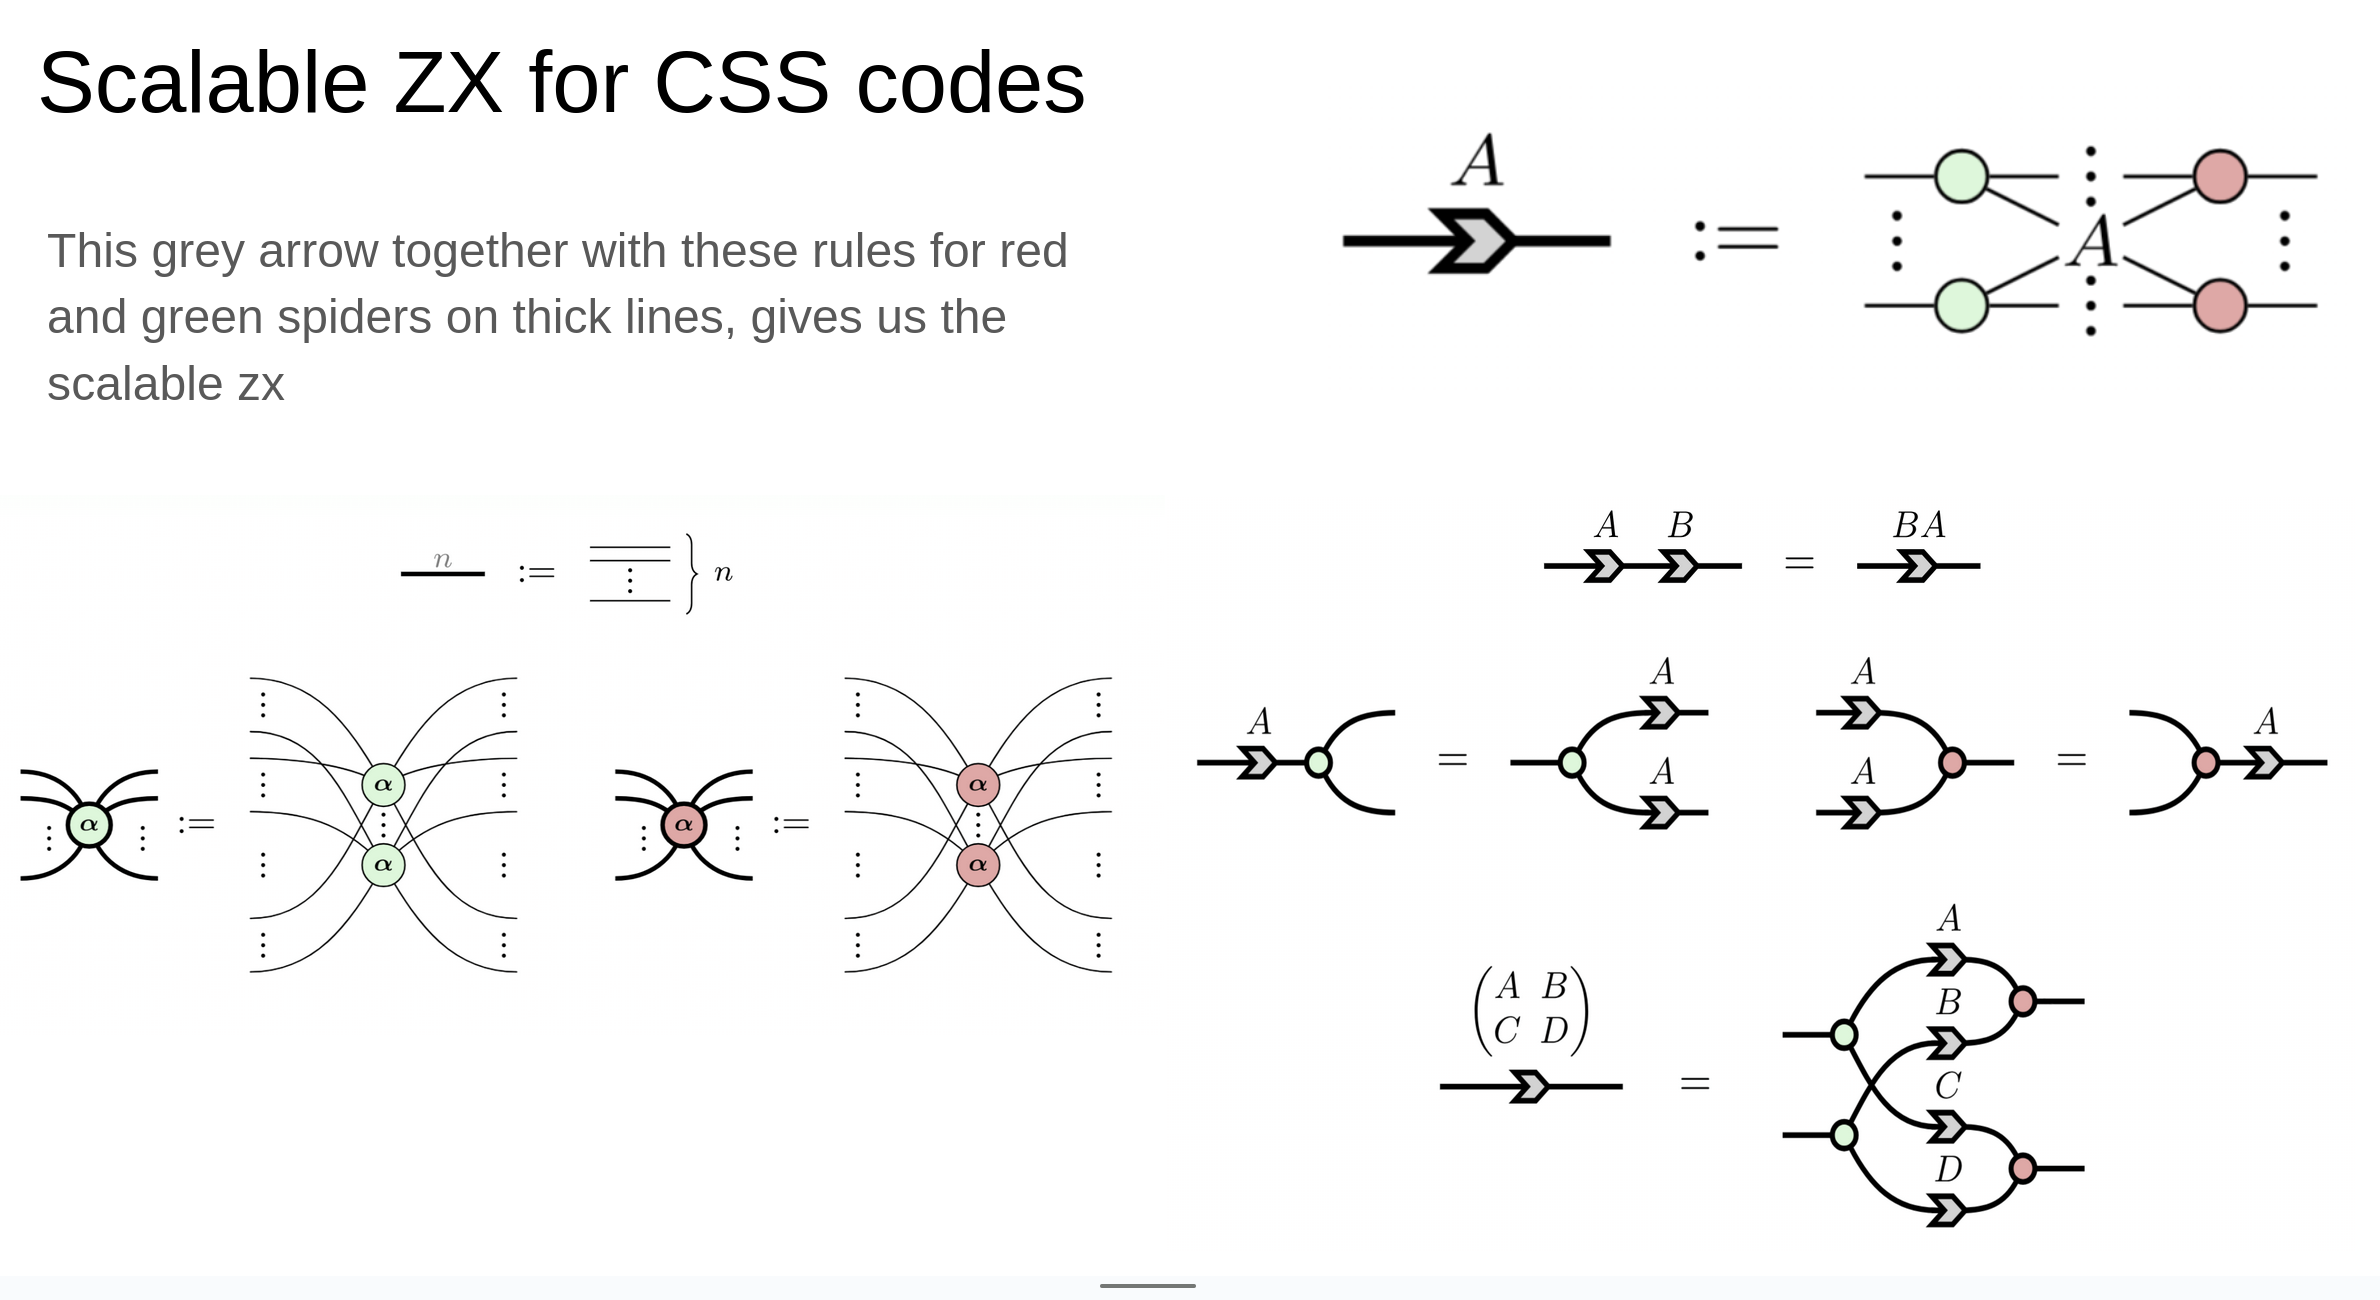
\includegraphics[width=\textwidth]{img/scalable2.png}
        % \caption{Here i want to point out the availability of scalable diagrams for structured scalable codes.}
    \end{figure}
\end{frame}

\begin{frame}
    \begin{figure}
        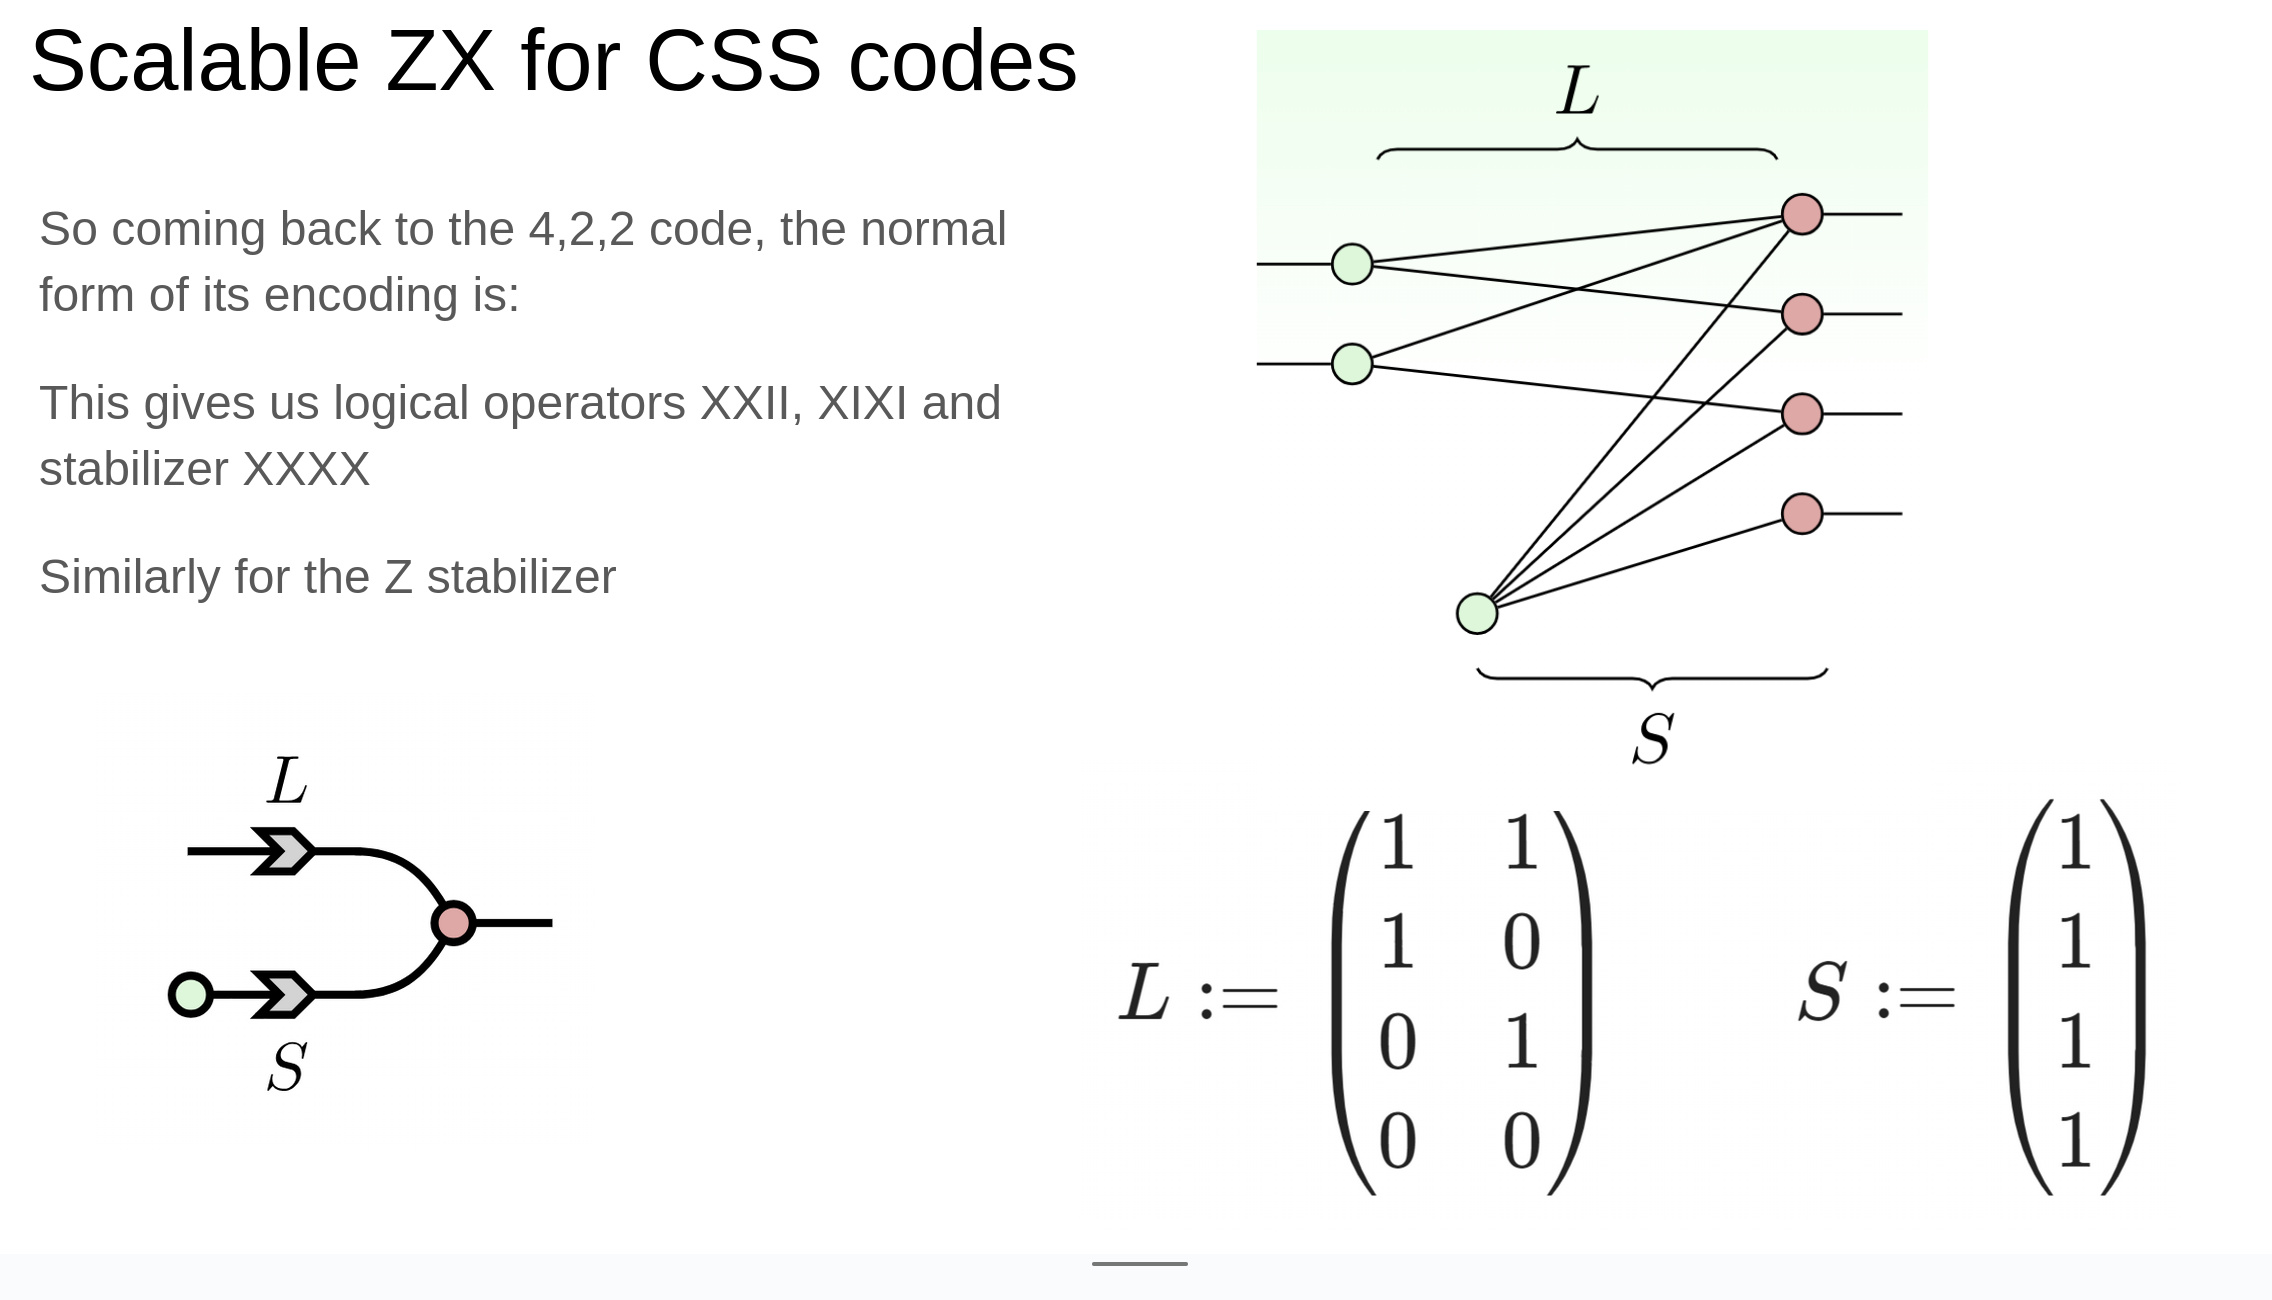
\includegraphics[width=\textwidth]{img/scalable.png}
        % \caption{Here i want to say more about nest identities in scalable ZX, like triorthogonal nest matrices being trivial}
    \end{figure}
\end{frame}



\begin{frame}
    \centering
    \vfill
    {\Large\itshape
    ``Physics is all about Symmetries.''\\[1em]
    \raggedleft -- Daniel Reich, Advanced Quantum Mechanics
    }
    \vfill
\end{frame}
% \begin{frame}
%     \centering
%     \vfill
%     {\Large
%     Thanks for listening!}
% \end{frame}
\begin{frame}{Sources}
    \begin{itemize}
        \item https://www.cs.ox.ac.uk/people/aleks.kissinger/papers/borghans-thesis.pdf
        \item https://arxiv.org/pdf/2410.17240
        \item https://arxiv.org/pdf/2212.04462
        \item "Picturing Quantum Processes" A.Kissinger & B. Coecke
        \item "Picturing Quantum Software" A.Kissinger & J. Van de Wetering
    \end{itemize}
\end{frame}


\end{document}